\documentclass[parskip]{cs4rep}

\usepackage{hyperref}
\usepackage{todonotes}
\usepackage{natbib}
\usepackage{subcaption}
\usepackage{amsmath}
\DeclareMathOperator*{\argmax}{arg\,max}
\DeclareMathOperator*{\argmin}{arg\,min}

\newcommand{\gene}[1]{{\tt #1}}
\newcommand{\histonemodification}[1]{#1}
\newcommand{\celltype}[1]{#1}

\begin{document}

\title{Clustering and Visualisation\\ of DNA Sequencing Data}

\author{Saulius Lukauskas}

\degree{Artificial Intelligence}
\project{Undergraduate Dissertation}

\date{\today}

\abstract{
\todo{Need an abstract}
}

\maketitle

%\section*{Acknowledgements}
%Acknowledgements go here.

\tableofcontents

%\pagenumbering{arabic}


\chapter{Background and Introduction}

The complete set of information required to create and maintain cells of a
living organism is contained in the genome of the organism. In humans, this
information is encoded in a long chain of nucleotides within the DNA molecules
in 23 different chromosomes located in the nucleus of every cell as well as in
a small segment of DNA located within the mitochondrion of the cell.  
These chains of nucleotides can be sequenced by determining the order of appearance
of the four bases within the genome: adenine (often abbreviated as simply "A"), cytosine (abbreviated as C),
guanine (G) or thymine (T).
The sequence of these nucleobases is commonly referred to as the DNA Sequence. 

\section{Structure of  DNA}
Generally DNA molecules are observed in pairs of two tightly connected
molecules, rather than as a single molecule. These molecules are known as
strands and are held together by the bonds between the nucleobases: guanine is
known to form a bond with cytosine, whereas adenine forms a bond with thymine.
Since each kind of nucleobase can form a bond with only one other kind of
nucleobase, both of the DNA strands contain enough information to recreate the
other on its own. This redundancy is required for DNA replication process. 

Because of this redundancy, the sequences on complimentary strands are often considered at the
same time as sequences of base pairs, rather than sequences of nucleotides. The
human sex cells are known to contain around three billion such base pairs.

\subsection{Histones}
\todo{Fill me in}
\subsection{Transcription and Splicing}
\todo{Need to explain here what are transcription start sites, exons and why they are important
as the remaining sections assume the reader is aware of them}

\section{Next-Generation Sequencing}
The Human Genome Project was the research project that has sequenced all
three billion of these base pairs for the first time. The project was estimated
to cost 3 billion dollars for American tax payers and last 15 years, but has ended up
costing a bit less than that - \$2.7 billion and was completed in 13
years\footnote{See \url{http://www.genome.gov/11006943} and
    \url{http://www.ornl.gov/sci/techresources/Human_Genome/project/about.shtml}
    for more information}. 
    
 Since then, a variety of DNA sequencing methods were
developed that reduce both the time and cost required to perform sequencing
significantly\citep{Shendure:2008uc,Liu:2012ve}. New technology and reduced
costs of DNA Sequencing has made it more accessible and allowed
development of new genome-scale analysis methods such as ChIP-Sequencing
(ChIP-Seq).

\todo{Unfinished}
\todo{Mention that NGS = Next Generation Sequencing}

\section{ChIP Sequencing}

\chapter{Motivation}
The amount of data collected from the next-generation sequencing is increasing rapidly together with the popularity of NGS. This data has already provided useful insights into the processes of living organisms, and it is expected that more and more such insights will be discovered as more data is obtained.\todo{find a few examples} 
Unfortunately, the more data is obtained, the harder the process of obtaining useful insights becomes.  
The title of one of the conference on NGS, where a poster about this project will be presented at, seems to summarises this problem well: "The Next NGS Challenge: Data Processing and Integration"\footnote{http://www.thenextngschallenge.org/}.

This trend seem to be following the prediction published in one of the early reviews of ChIP-Seq, \cite{Park:2009wc}, where P J Park already predicted data processing to be the major challenge of this technology. In this paper, he listed the common approaches to data processing at that time, most of which are still valid today.

For protein-DNA binding, he writes, the most common analysis is the discovery of binding sequence motifs. A large variety of methods in doing that are available to this day, probably the best-known one being MEME\cite{Grundy:1997vb}. In order to find these transcription factor binding sites, significantly enriched regions of the genome (so called "peaks") need to be located first. A variety of methods exist to aid this task. The probably best-known of them, MACS peak caller\cite{Zhang:2008wp}, has been used in one of the experiments performed for this project (\autoref{sec:macs-experiment})\todo{Explain how macs works if there is time}. Other methods of finding these enriched regions are summarised in a more recent review on ChIP-SEQ\cite{Furey:2012ha}.

For histone modifications, as claimed by P J Park, an obvious approach is to annotate the locations of these peaks relative to known genomic features. For instance, such analysis would record the fact that \histonemodification{H3K4me3} tends to be enriched near transcription start sites, as discussed earlier\todo{Discuss earlier}. Then these annotated regions need to be analysed either by looking for correlations, or by advanced clustering techniques. 

One of the early clustering methods, referenced by Park, is ChromaSig\cite{Hon:2008wv}. The authors claim their method is able to identify the motifs previously defined by \cite{Heintzman:2007ke} near well-defined genomic regions (e.g. transcription start sites) in a completely unsupervised way. 
A bit more recent approach, \cite{Lai:2010ue}, uses a similar method to find the best alignment between 
a set of user-defined regions. 

These methods share a major weakness of being window-based.
Window-based methods are not able to identify similar patterns if they differ in length. Bieberstein and colleagues, have shown an example of such pattern. They found that \histonemodification{H3K4Me3} profiles tend to peak at the locations of first splicing sites of genes\cite{Bieberstein:2012tf}. Since the locations of first splice site relative to transcription start sites vary from one gene to another, methods that do not model this are deemed to fail identifying that these peaks at the splicing sites are related.

Also, in some cases, using a window-based approach does not make any sense at all. For instance, if one was comparing genes, which differ vastly in length, it makes little sense to compare the full length of one gene, to a small part of some other gene. This is the reason why some studies, e.g. \cite{Taslim:vj}, rescale the regions of interest to be of the same length, before doing clustering. This could indeed detect similar patterns that vary in length, however such approach is vulnerable to misalignment -- a problem window-based alignment methods solve pretty well.

An interesting approach on this problem is taken by Wang et al.\citep{Wang:2012cb}. 
Their method is based on the methods developed for sequence alignment.
The algorithm they propose, ChAT, tries to find the best alignment between two patterns before doing any clustering, just as ChromaSig or ArchAlign, yet it allows to ignore a part of some region as if it was not there. The authors of the paper claim that these gaps "are critical because they allow the algorithm to extend beyond regions with variant (or diffuse) chromatin enrichment signatures, and in so doing facilitate the discovery of chromatin signatures that span long genomic regions as well as those with complex multi-modal patterns of histone modification enrichment". 

This, in fact, is a very similar approach to the one taken in this project. The main difference is that when creating gaps, ChAT algorithm applies a penalty that is proportional to the norm of the vector that is being skipped. Such penalty biases the algorithm to skip unexpressed regions more than expressed ones as per reasoning that depleted regions are not as interesting as the expressed ones. 
While this penalty allows the discovery of multi-modal patterns separated by depleted regions across genome as the authors claim, it would heavily penalise any attempts to discover highly-expressed patterns of varying lengths.

The intuition behind the methods proposed in this project comes from realising that the problem of comparing genomic marks is a problem that is very similar to comparing waveforms for speech recognition. That is, in speech recognition, we want to identify two words being the same even though we started recording one of them, say half a second later, which is equivalent of detecting patterns that are similar, but misaligned. Similarly, if one speaker was to say the same word faster than the other, what is equivalent to comparing genomic regions of different lengths, the words should still be detected as being the same. A common solution for this problem in Speech Recognition community is to use Dynamic Time Warping distance to compare the waveforms.

Contrary to the ChAT method, this distance measure does not allow skipping of points at all. It does, however, allow a set of points on one sequence to a single point on another as if that point was stretched to become a sequence of n points. This way the penalty of warping the genome depends directly on the points that are mapped together, so the algorithm is able to do this both for highly-expressed and depleted regions, as long as the values mapped to each other are similar. See methods section for an in-depth overview of this.

\todo{Talk about CAGT a little bit. From what I understand their tool is focused on reversing the patterns correctly. If this is true, the need to add the reversing next to aims of this project, if not then it need not be here.}

\todo{Mention the two major papers in the game}

\chapter{Methods}
\section{Dynamic Time Warping}

\begin{figure}[b,t]
   \centering
   \begin{subfigure}[b]{0.45\textwidth}
       \centering
       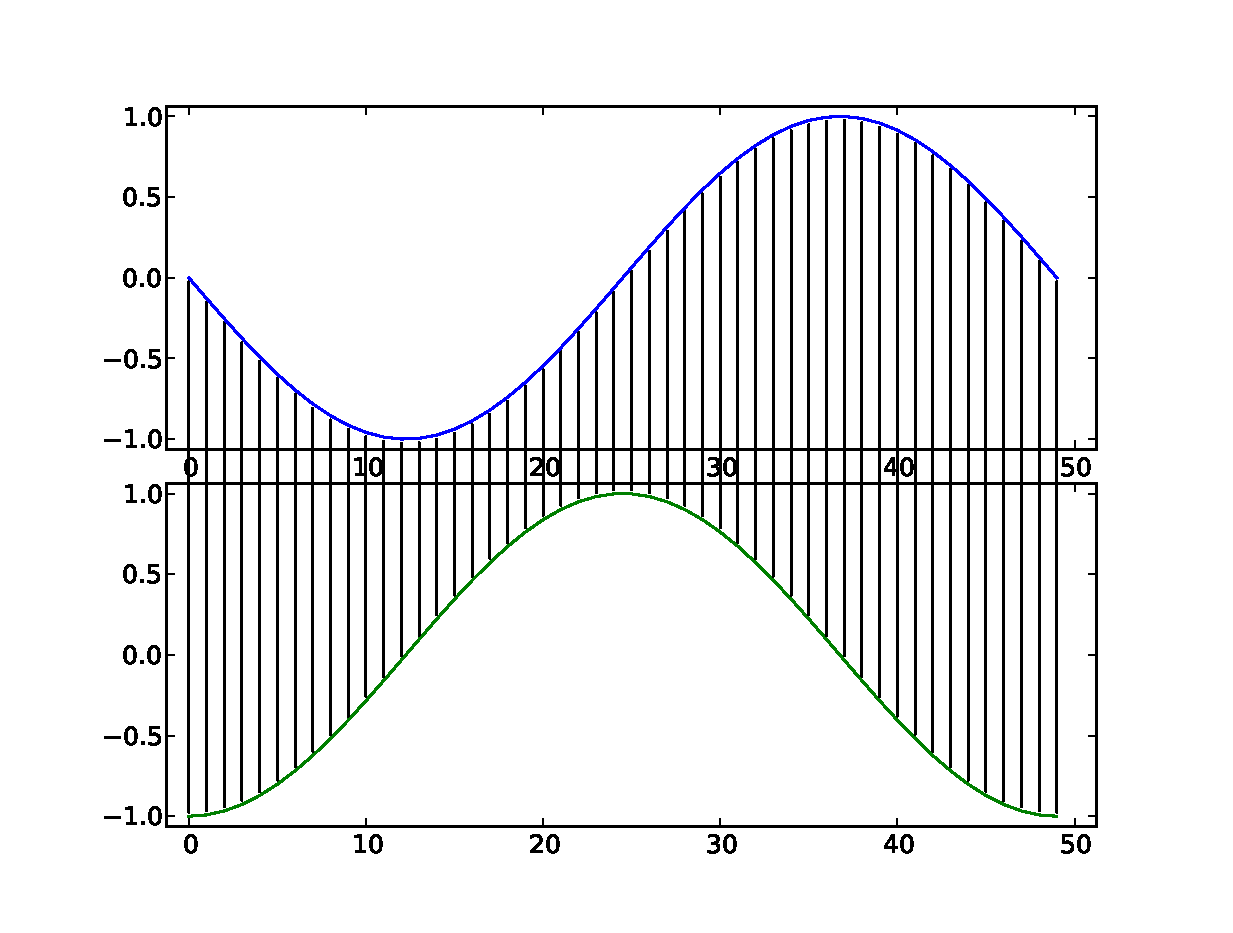
\includegraphics[width=\textwidth]{figures/DTW/sin-cos-no-dtw.eps}
       \caption{Euclidean alignment}
       \label{fig:DTW:euclidean_alignment}
   \end{subfigure}
   ~
   \begin{subfigure}[b]{0.45\textwidth}
       \centering
       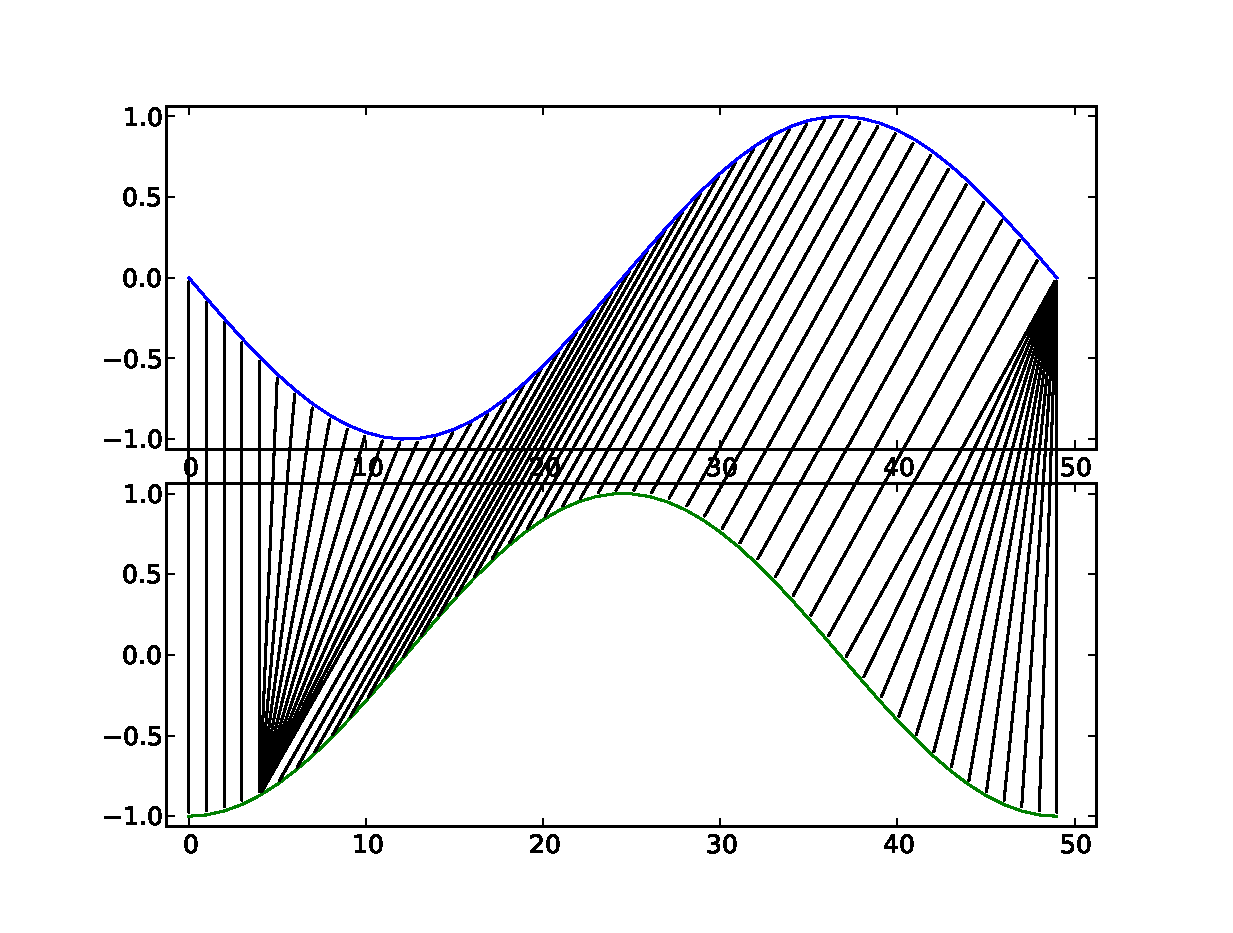
\includegraphics[width=\textwidth]{figures/DTW/sin-cos-dtw.eps}
       \caption{DTW alignment}
       \label{fig:DTW:dtw_alignment}
   \end{subfigure}
   
   \caption{Two sequences aligned to each other. Figure \ref{fig:DTW:euclidean_alignment} maps each point on sequence A to a point on sequence B directly, resulting in an Euclidean distance measure, whereas figure \ref{fig:DTW:dtw_alignment} uses Dynamic Time Warping algorithm to find a better mapping between the points.}
   \label{fig:DTW:alignments}
\end{figure}


Dynamic Time Warping (DTW) algorithm is the corner stone of the methods implemented in this project. This algorithm was initially developed in the speech recognition community in order to allow accurate comparisons between words spoken with tempo variations. 
This comparison is achieved by warping the time axis nonlinearly. That is, the axis is stretched or compressed as to minimise the total distance between the points aligned to each other. The stretching and compressing is done by creating an alignment between the two sequences, also known as the warping path, almost arbitrarily, with a few constraints described below. The distances between aligned points are then computed and summed to obtain what is commonly referred to as DTW Distance.

More formally, given two sequences $\mathbf{a} = a_1, a_2, ..., a_n$ and $\mathbf{b} = b_1, b_2, ..., b_m$, Dynamic Time Warping aims to construct a warping path $\mathbf{p} = { (p_{1,0}, p_{1,1}), (p_{2,0}, p_{2,1}), ..., (p_{k,0}, p_{k, 1}) }$ that maps each point on the first sequence, specified as $p_{i,0}$ to a point on the second sequence, $p_{i,1}$ such that the following three constraints hold:

\begin{enumerate}
\item \emph{Boundary Condition}: The path must start at the first point of sequence $\mathbf{a}$ and this point must be mapped to the first point of the second sequence: $p_1 = (1,1)$. Similarly, the final points of both sequences should be mapped to each other, and the path must end there: $p_k = (m, n).$ 
\item \emph{Monotonicity Condition}: The path must not move \emph{back in time}: 
    $p_{1,i} \le p_{2,i} \le p_{3,i} \le ... \le p_{k, i}$ for both $i=0$ and $i=1$.
\item \emph{Step Size Condition}: At each step the path must either map the same point on one sequence to the next point on another sequence, or map next points on both sequences together, mathematically:
    $p_{i+1} - p_{i} \in \{(0,1), (1,0), (1,1)\}$ for all $i < k$.
\end{enumerate}

Furthermore, we are only interested in a warping that is minimal, given some distance measure $d$ that would compute the distances between aligned points (e.g. Euclidean distance): $\hat{P} = \argmin_P \sum_{(i,j) \in P} d(a_i, b_j)$. Such minimal warping alignment can be computed in $O(nm)$ time by applying dynamic programming techniques. We construct a $n \times m$ matrix $\mathbf{D}$ where each entry $D_{i,j}$ will contain a minimal (warped) distance of matching first $i$ components of the first sequence, $a_1..a_i$, to first $j$ elements of the second sequence, $b_1..b_j$. The first component of the matrix, $D_{1,1}$ is initialised to the distance between the first components of the two sequences, $d(a_1, b_1)$ as specified by the boundary condition.

The matrix is then filled row by row, according to the following recursive equation:
$$D_{i,j} = d(a_i, b_j) + min(D_{i-1, j}, D_{i, j-1}, D_{i,j})$$

In the end, the column $D_{n,m}$ holds the minimal warped distance between two series.
If the minimal warping path is needed, it can be traced back by following the recursive relation backwards from $D_{i,j}$. Please refer to \citep{Muller:2007bo} for more details on the workings of DTW.

To illustrate what DTW does, have a look at the \autoref{fig:DTW:alignments}. The two sequences in the figure are sine and cosine plotted over the range $[-\pi; \pi)$. Given the nature of these functions, we know that the shapes in the two sequences are essentially identical, just shifted by $\frac{\pi}{2}$ radians, therefore we should get a good alignment of them by some warping of the x axis that is used as the time axis in this sense.

In \autoref{fig:DTW:euclidean_alignment}, each point on the sequence A is aligned to corresponding point on the sequence B. If we were to sum the distances between aligned points, we would get the Euclidean distance between these two sequences. We can see that these sequences will likely not be labelled as similar, because the distance between mapped points is always large. The mapping seen in \autoref{fig:DTW:dtw_alignment}, on the other hand is able to correct for the shift in the X axis. 
The highest points are now mapped to each other, so are the other points that are in the patterns existing in both of the sequences. If we were to calculate the differences between the mapped points again, we would see that the resulting distance is much smaller than Euclidean one and the two sequences will likely be considered close, yet not identical, as there still are features in the sequence A that are not in the sequence B, for instance, the valley in the beginning, therefore resulting in a costly mapping between the two.

\subsection{Constrained DTW}

\begin{figure}
   \centering
   \begin{subfigure}[b]{0.45\textwidth}
       \centering
       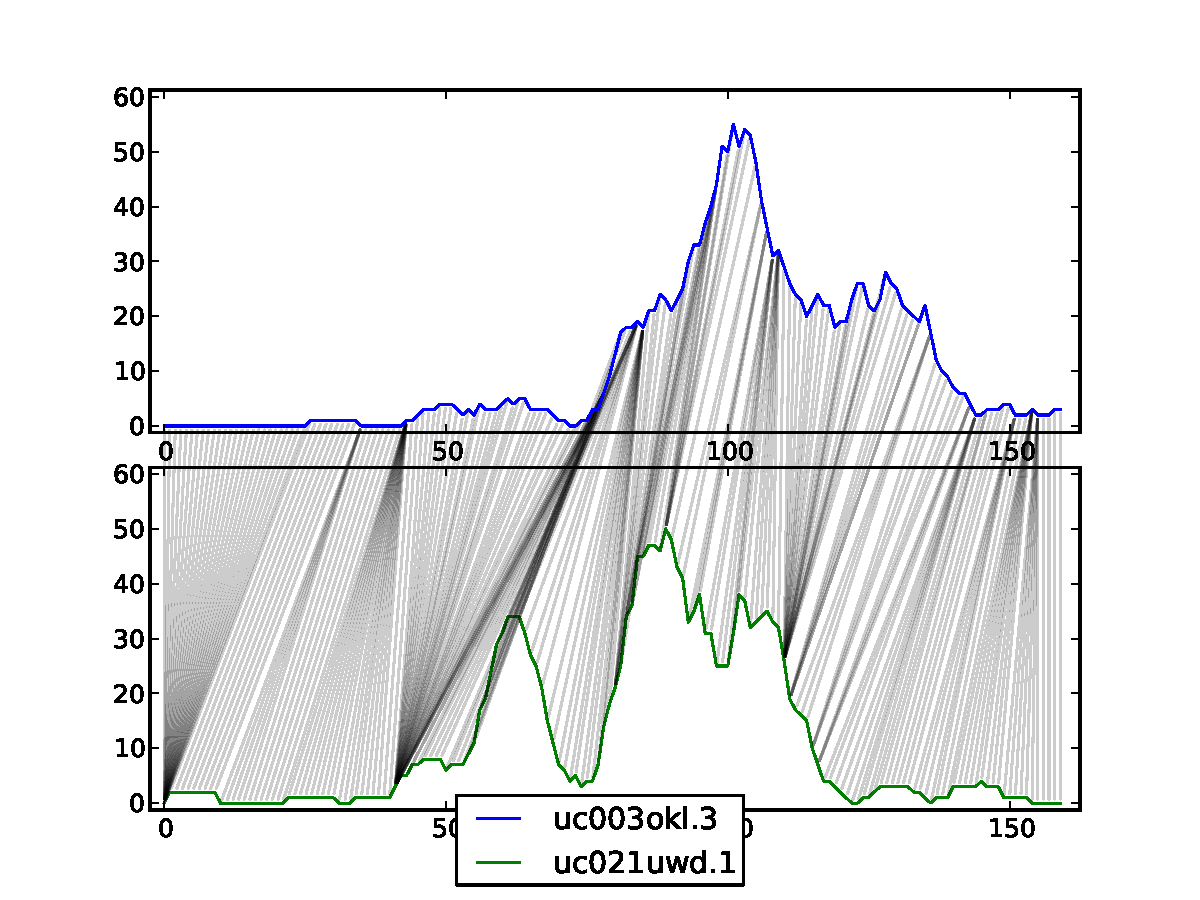
\includegraphics[width=\textwidth]{figures/DTW/uc003okl_3-uc021uwd_1-mappings-std.pdf}
       \caption{Alignments}
       \label{fig:DTW:std:mappings}
   \end{subfigure}
   ~
   \begin{subfigure}[b]{0.45\textwidth}
       \centering
       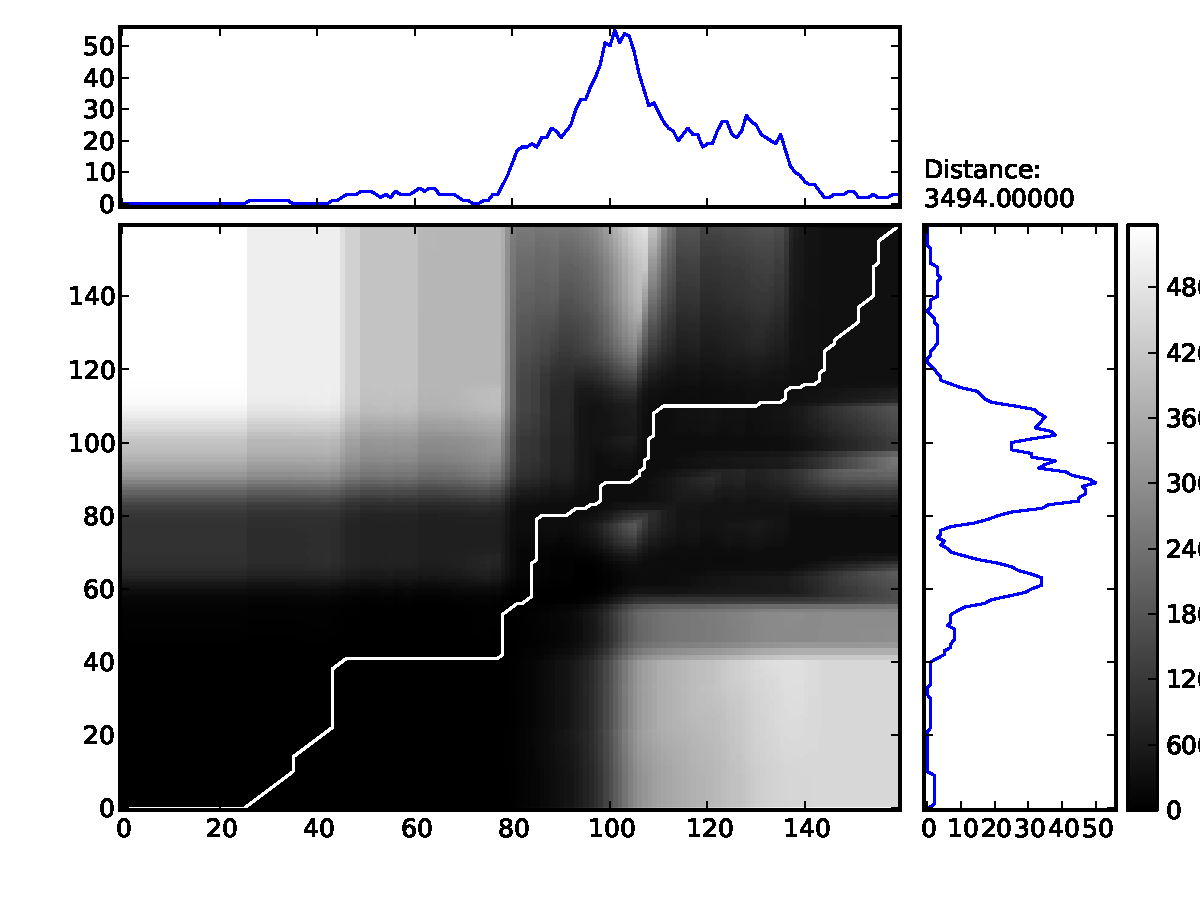
\includegraphics[width=\textwidth]{figures/DTW/uc003okl_3-uc021uwd_1-cost-std.pdf}
       \caption{Cost matrix and path}
       \label{fig:DTW:std:cost}
   \end{subfigure}
   \caption{Result of DTW distance calculation on the \histonemodification{H3K4Me3} Activation profiles around transcription start sites for two genes,  \gene{uc003okl.3} and \gene{uc021uwd.1}.}
   \label{fig:DTW:std}
\end{figure}
\todo{Make sure to explain what gene names mean}

In some cases, warping the time axis arbitrarily might not necessarily be a correct thing to do.
For instance, have a look at \autoref{fig:DTW:std}. Here DTW is used to compare the \histonemodification{H3K4Me3} activation profiles around transcription start sites (TSS) of two genes, \gene{uc003okl.3} and \gene{uc021uwd.1}. We can immediatelly see that first activation profile appears to be unimodal, whereas the second one is clearly bimodal. The minimal warping path maps a relatively inactive region from around bin 40 to around bin 80 in the series for \gene{uc003okl.3} to a single point on the series for \gene{uc021uwd.1}. However, this unexpressed region might have biological significance, e.g. \todo{double check if this is actually true} indicate removal of a nucleosome and we might not want to allow it to be compressed to a single point. 

We can manually impose restrictions on warping paths that are allowed by introducing global constraints. The two most commonly used global constraints on DTW are Sakoe-Chiba Band and Itakura parallelogram\citep{Ratanamahatana:2004wu}.

\subsubsection{Sakoe-Chiba Band}

\begin{figure}
   \centering
   \begin{subfigure}[b]{0.45\textwidth}
       \centering
       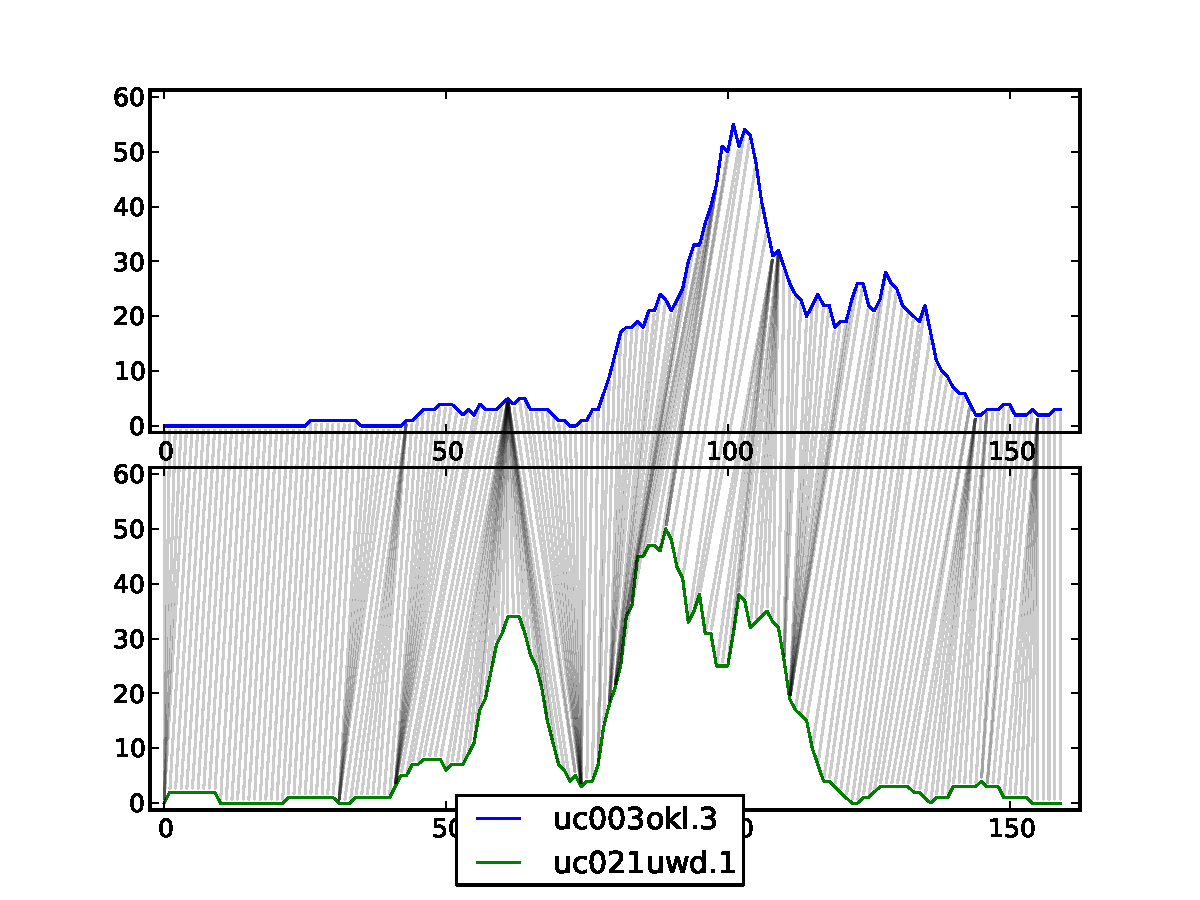
\includegraphics[width=\textwidth]{figures/DTW/uc003okl_3-uc021uwd_1-mappings-sakoe-chiba.pdf}
       \caption{Alignments}
       \label{fig:DTW:sakoe_chiba:mappings}
   \end{subfigure}
   ~
   \begin{subfigure}[b]{0.45\textwidth}
       \centering
       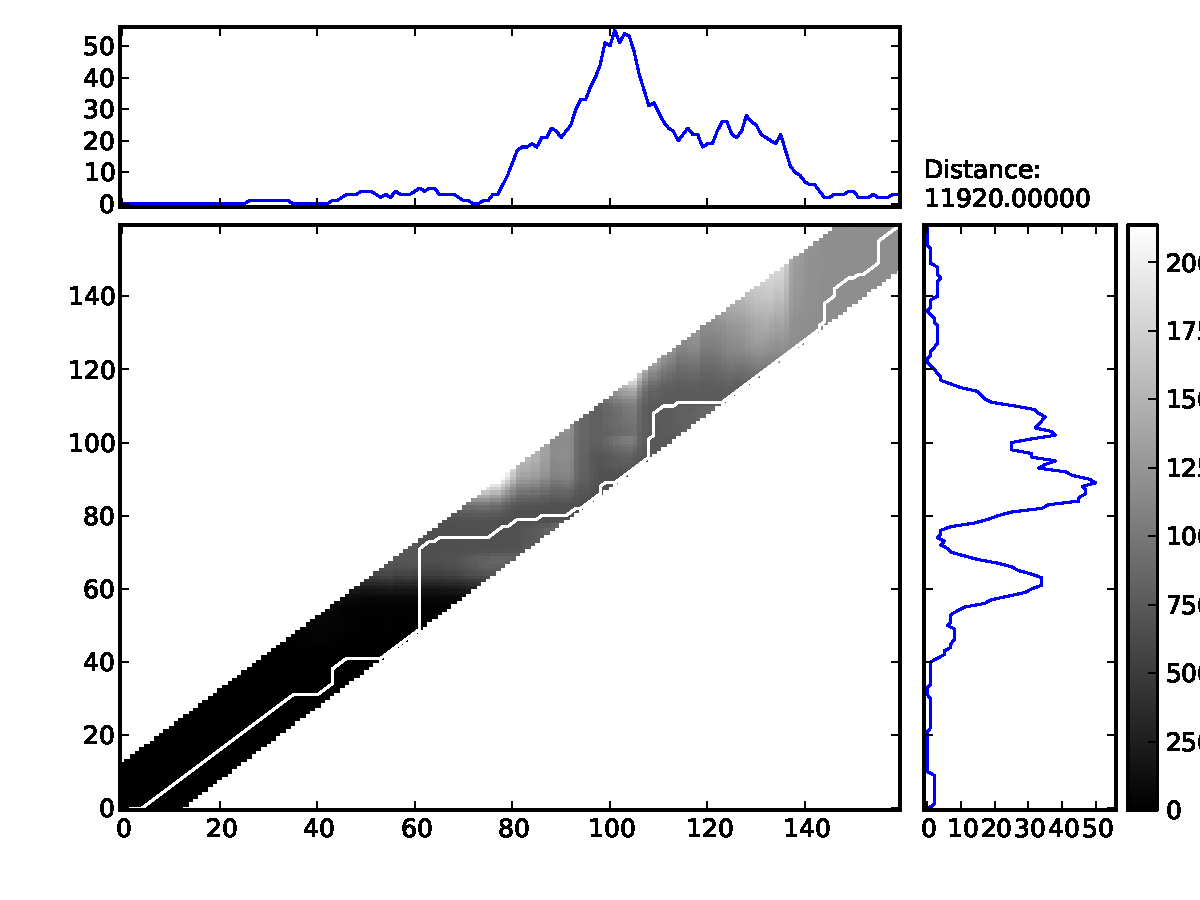
\includegraphics[width=\textwidth]{figures/DTW/uc003okl_3-uc021uwd_1-cost-sakoe-chiba.pdf}
       \caption{Cost matrix and path}
       \label{fig:DTW:sakoe_chiba:cost}
   \end{subfigure}
   \caption{Result of DTW distance calculation on the \histonemodification{H3K4Me3} Activation profiles around transcription start sites for two genes, \gene{uc003okl.3} and \gene{uc021uwd.1}. The DTW distance was constrained with Sakoe & Chiba constraint with $k = 12$.}
   \label{fig:DTW:sakoe_chiba}
\end{figure}

Sakoe \& Chiba constraint, as first described in \citep{Sakoe:1978ta} allows only the warping paths 
that satisfy $|i-j| \le k$ where $k$ is some integer specifying the tightness of the constraint. The constraint is commonly referred to as "Sakoe \& Chiba band" as the cost matrix looks like a band around the main diagonal (see \autoref{fig:DTW:sakoe_chiba:cost}). Such constraint reduces the complexity of DTW to $O(k \times max(n,m))$ where $n$ and $m$ are the lengths of the two sequences. 

Intuitively, the constraint requires that each point on sequence A is mapped to a point no more than $k$ points away on the sequence B. That is, it assumes that there won't be any warping of the time axis greater than by $k$ points. Note that setting the $k$ parameter to zero would give us Euclidean distance between the two sequences.

\autoref{fig:DTW:sakoe_chiba} compares the same regions in the \autoref{fig:DTW:std} using the DTW constrained with Sakoe \& Chiba band of length $k=12$. One can see that the peaks on the right-hand side of the two sequences are still aligned correctly, but the relatively inactive region in the first sequence is now forced to be mapped to the left peak in the second sequence, resulting in a huge cost penalty and making the sequences quite distant from each other. This alignment results in a total distance of 11920 using squared euclidean distance as the local distance measure. Compare that to the distance of 3494 obtained by unconstrained warping.

As far as the author is aware, there is no established way of picking the value of parameter $k$.
Historically, $k$ was set to 10\% of the length of the sequences.
For nearest-neighbour classification tasks, \cite{Ratanamahatana:2004wu} has shown that an even a window sufficiently smaller than 10\% gives the highest accuracy for some datasets, though the actual number strongly depends on the actual dataset. Due to this, the constraint $k$ is not imposed in the Dynamic Genome Warping package and is left as a free parameter an user could specify herself.

\subsubsection{Slanted Band Constraint}
\label{sec:slanted-band-constraint}

Sakoe \& Chiba band makes DTW incomputable for sequences whose lengths differ by more than $k$ items, as the last points of those sequences point $n$ and point $m$ will not satisfy the constraint 
$|i-j| \le k$. The reason for this failure is the fact that $i=j$ is not the real diagonal of the cost matrix if the lengths of the two sequences, $n$ and $m$, are not equal. 
Toni Giorgino \nocite{Giorgino:2009ue} was well aware of this problem when implementing DTW module for R \footnote{The R Project For Statistical Computing - \url{http://www.r-project.org/}} where he included a modified version of Sakoe \& Chiba constraint, he calls a slanted band constraint\citep{Giorgino:2009ue}. 

Slanted band constraint solves the problem of different sequence lengths by changing the constraint to 
$|i - \frac{m}{n} \times j| <= k$, where $m$ and $n$ are the lengths of the two sequences being compared. This essentially changes the slope of the diagonal line to $\frac{m}{n}$ (cf. to slope being 1 in \citep{Sakoe:1978ta}). Unfortunately, the meaning of the parameter $k$ is inconsistent in this definition: if the second sequence is longer than the first one, thus $m > n$, the constraint can be thought to scale the second sequence down to the length of the first one and then apply the Sakoe \& Chiba constraint of size $k$, meaning $k$ is in the units of the shorter sequence. However, if the second sequence is shorter than the first one, it will be essentially rescaled to match the length of the first (longer) sequence and then the parameter $k$ will be measured in units of the longer sequence. In this particular case, DTW distance might not even be computable as in order for the warping path to remain continuous, the following inequality must hold $(j+1) \frac{m}{n} - k \le j \frac{m}{n} + k + 1$. In other words, for each $j$, there should be some $i$ in the warping window, that is either in the window of $j+1$ or is by at most one unit away from some $i'$ that is. Reshuffling the inequality we get that this holds if $\frac{m}{n} \le 2k + 1$ does.

This inconsistency might not be important in the situations where we have a query sequence that we want to match to a reference sequence as the order of parameters will not change in these cases. However, other applications, such as clustering, require symmetry. Since DGW uses DTW distance for clustering, I had to solve these issues with slanted band constraint, thus
DGW implements a modified version of it. 

The new constraint always assumes that the first sequence is longer than the second one. The slope parameter is again calculated as $s = \frac{m}{n}$, however it is now always less than or equal to one. This slope this slope is now applied to the first sequence, (not the second one as in \citep{Giorgino:2009ue}) essentially scaling it down to the length of the shorter sequence, giving the constraint: $|\lceil i \times \frac{m}{n} \rceil - j| \le k$. The algorithm could be modified and the slope applied to the second sequence instead, of course, however, the implementation is a bit more intuitive if it is the first sequence that gets rescaled not the second. 

This modified constraint is now always consistent, being in units of shorter sequence, and defined for all possible sequences.

\subsection{Constant-Penalty DTW}

\section{Clustering}

Centroid based clustering methods, e.g. K-Means, require a notion of centroid for data points being averaged. Centroid is usually defined as a data point that minimises the distance to all other data points in the set. In the Euclidean space this problem is trivial and solvable by calculating the mean of the data.

In the Dynamically Time Warped space, however, finding the centroid sequence, called a Steiner sequence, is a NP complete problem as the search space grows exponentially to the number of sequences\cite{Hautamaki:2008fh,Petitjean:2012bp}.

The fact that DTW distance does not satisfy the triangle inequality, \cite{Muller:2007bo}, 
is one of the reasons why this is such a hard problem. Various approximations for shape averaging were
proposed throughout the years, some of them can be find in, e.g. \cite{Niennattrakul:2009ep}\cite{Petitjean:2011bq}\cite{Petitjean:2012bp} \todo{Okay, i wont do this today as my mind is on the results section, do this some other time when you can do it properly}

\todo{Complete linkage}

\section{Biologically Relevant Heuristics}
\todo{Write about antisense regions correction}

\chapter{Implementation Details}
\todo{Mention and cite all the libraries DTW builds on}

\section{File formats}
\subsection{BAM}
\subsection{BED}
  
\section{Time Complexity}
\subsection{Native-C Modules}
\subsection{Parallel processing}
\todo{Write about how expensive DTW is, write about what a pain is to do multiprocessing it in Python}

\chapter{Results}
Evaluation of results of clustering methods has always been a challenging problem. Since clustering, by definition, is unsupervised, there hardly is any ground truth on what the correct way of assigning data into clusters is. Some cluster assignments might be desired in some applications, others might be desired in completely different applications. Furthermore, there is the problem on where to cut the hierarchical clustering dendrogram at, \todo{Discuss this}that has already been discussed.

\section{Clustering an Artificial Dataset}
One way to estimate the performance of the clustering is by performing it on a dataset known to have some \emph{a priori} groups. In the spirit of the paper claiming that first exon length influences the H3K4Me3 mark around the Transcription Start Sites\cite{Bieberstein:2012tf}, a test dataset randomly stretching the exons of known transcription start sites was generated.

More precisely, 5 random transcription start sites that have their first exon in the window of 2000 base pairs were chosen. \todo{The sites were chosen as to pass --min-pileup constraint, add this if I explain about min pileup somewhere before} The data for these windows around the transcription start sites was read at the resolution of 25 base pairs per bin. 

The regions where first exons lie were extended randomly to be up to 60 bins longer (that's up to $60x25=1500$ base pairs longer). The extension was performed by repeating the bins uniformly in the same order as to obtain the same mark within the exon, just stretched. A new dataset of size 500 was generated by performing these random permutations on the 5 seed regions. 
These newly-generated regions were then randomly mutated, with probability of $0.33$, by changing a value of a data point, to some random value picked from the uniform distribution $U(0.5x, 1.5x)$ where $x$ is the previous value of the point. These newly-generated regions were then randomly reversed with probability of 50\% to generate data for antisense patterns.


\begin{figure}[t,b]
    \centering
    \begin{subfigure}[b]{0.3\textwidth}
        \centering
        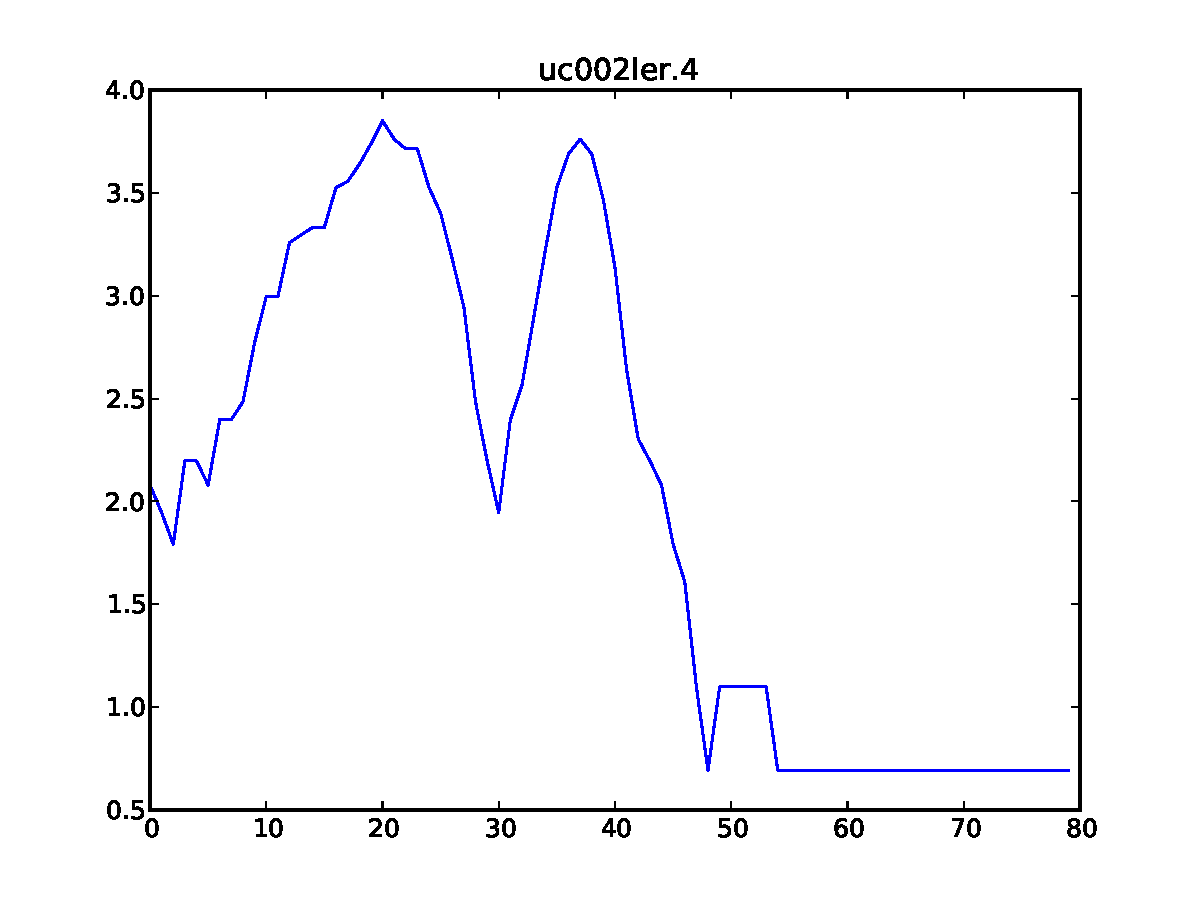
\includegraphics[width=\textwidth]{figures/evaluation/exon_stretching/uc002ler_4.pdf}
        \caption{\gene{uc001ler.4}}
        \label{fig:evaluation:exon_stretching:seeds:a}
    \end{subfigure}
    ~
    \begin{subfigure}[b]{0.3\textwidth}
        \centering
        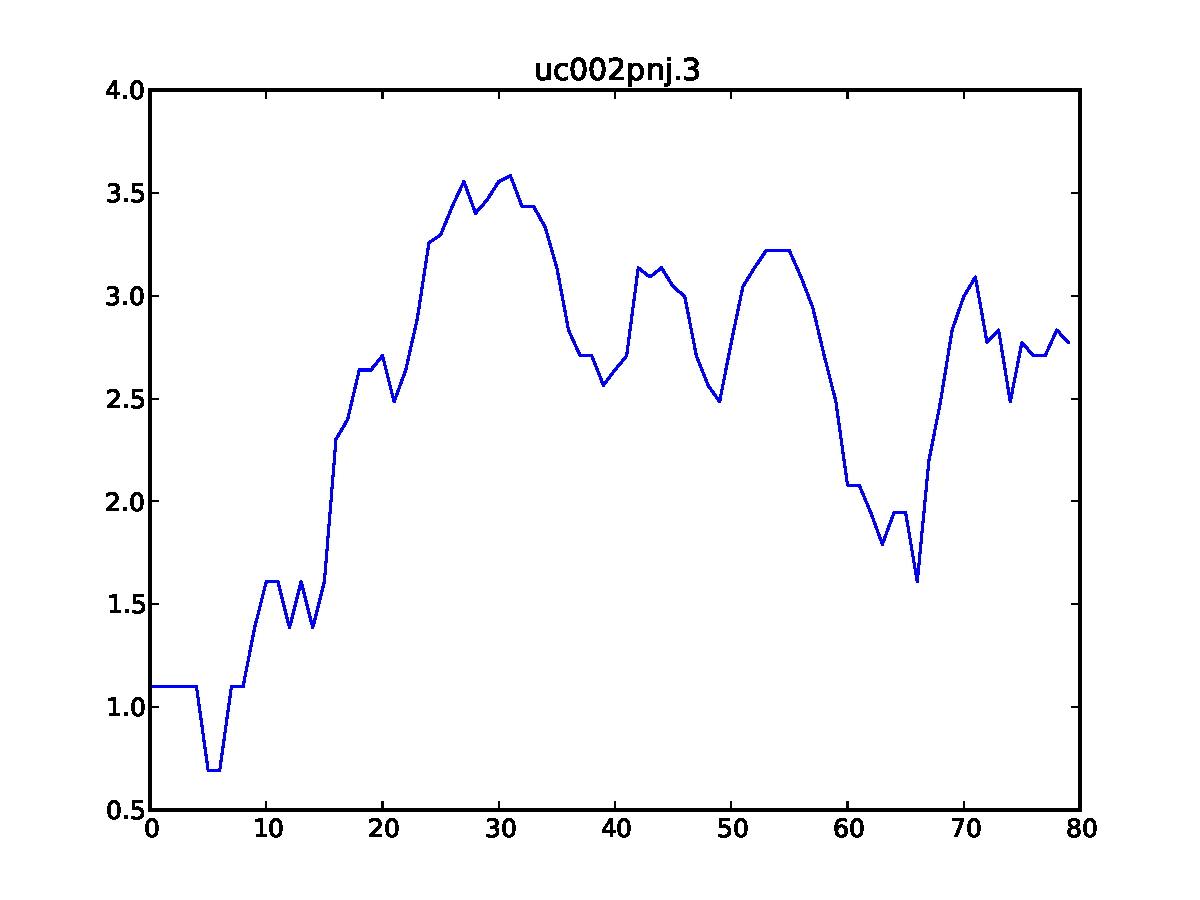
\includegraphics[width=\textwidth]{figures/evaluation/exon_stretching/uc002pnj_3.pdf}
        \caption{\gene{uc001pnj.3}}
        \label{fig:evaluation:exon_stretching:seeds:b}
    \end{subfigure}
    ~
    \begin{subfigure}[b]{0.3\textwidth}
        \centering
        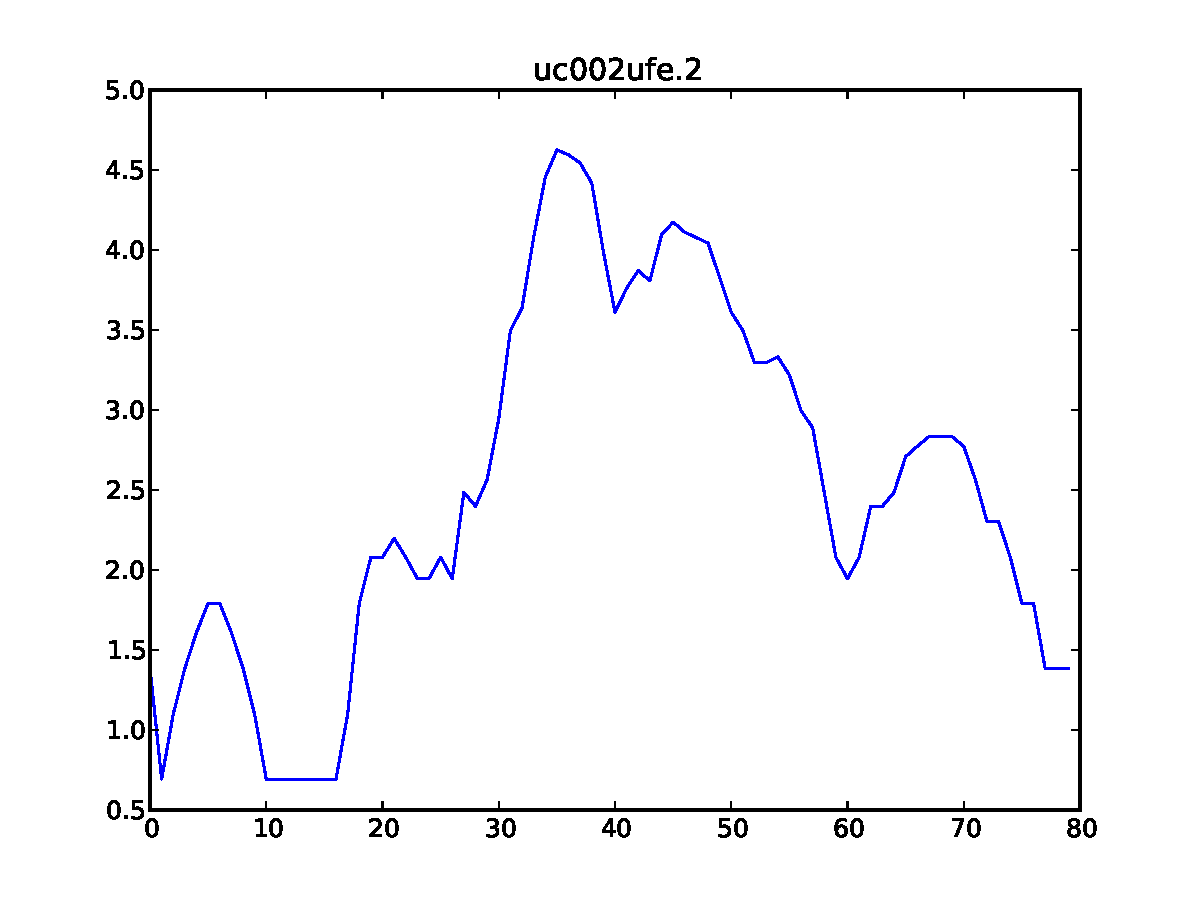
\includegraphics[width=\textwidth]{figures/evaluation/exon_stretching/uc002ufe_2.pdf}
        \caption{\gene{uc001ufe.2}}
        \label{fig:evaluation:exon_stretching:seeds:c}
    \end{subfigure}
    ~
    \begin{subfigure}[b]{0.3\textwidth}
        \centering
        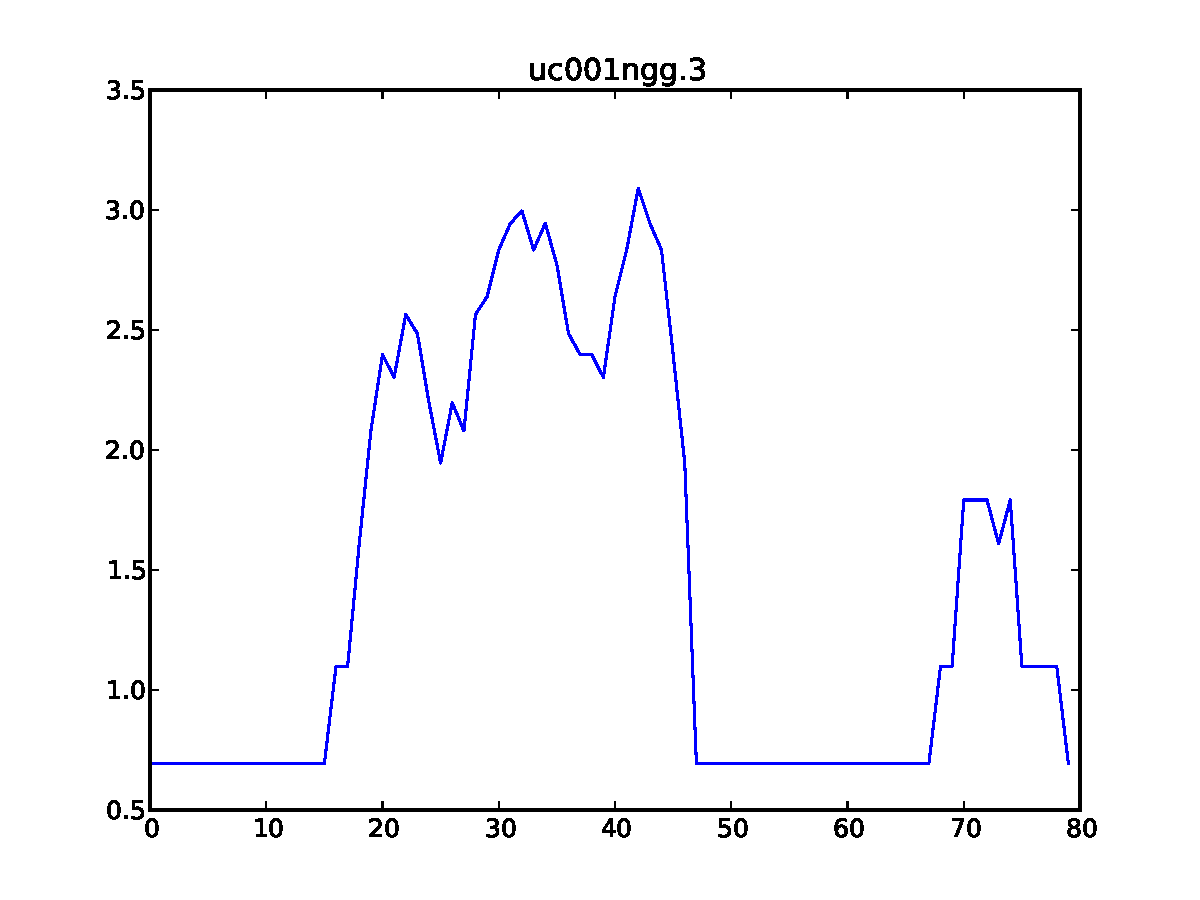
\includegraphics[width=\textwidth]{figures/evaluation/exon_stretching/uc001ngg_3.pdf}
        \caption{\gene{uc001ngg.3}}
        \label{fig:evaluation:exon_stretching:seeds:d}
    \end{subfigure}
    ~
    \begin{subfigure}[b]{0.3\textwidth}
        \centering
        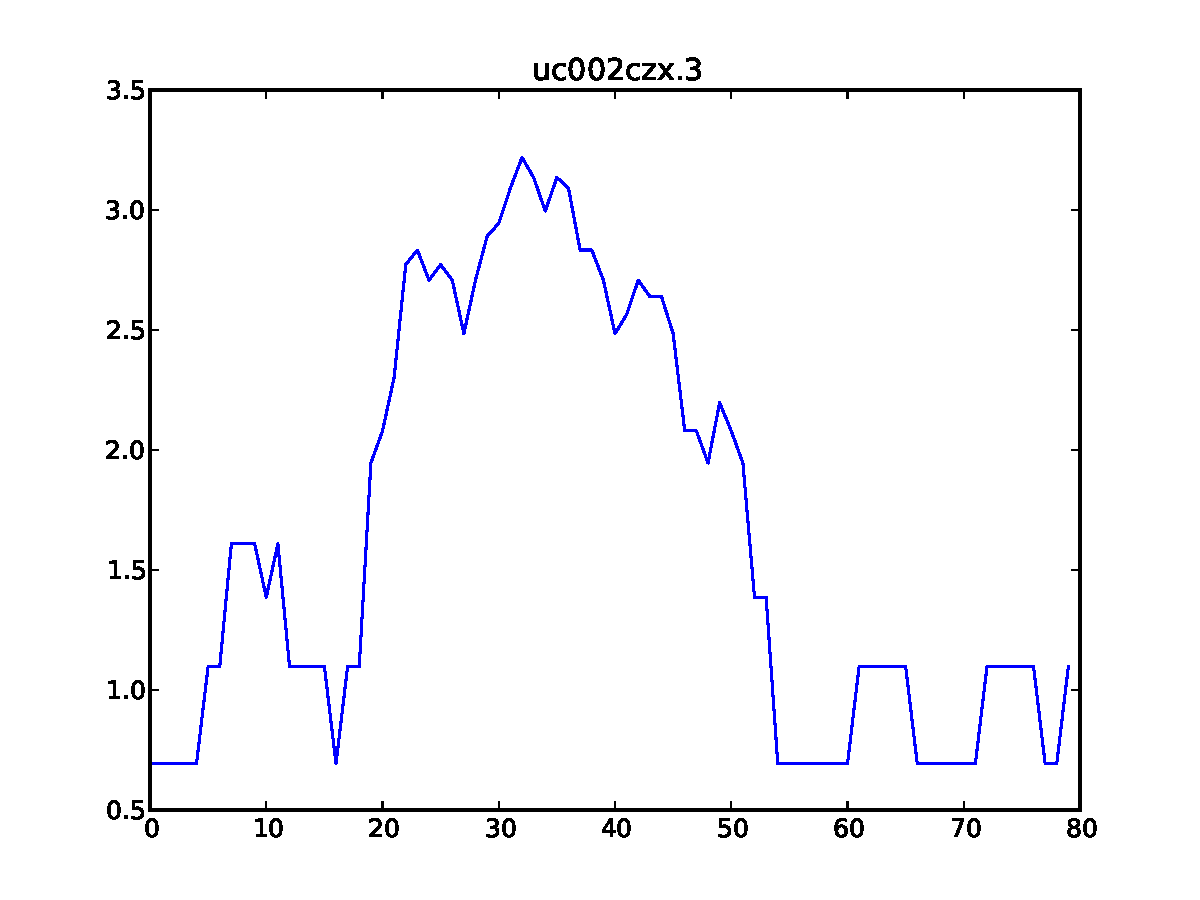
\includegraphics[width=\textwidth]{figures/evaluation/exon_stretching/uc002czx_3.pdf}
        \caption{\gene{uc001czx.3}}
        \label{fig:evaluation:exon_stretching:seeds:e}
    \end{subfigure}
    \caption{The five seed regions that were used to create the manual dataset. Note how similar the the patterns in \ref{fig:evaluation:exon_stretching:seeds:d} and \ref{fig:evaluation:exon_stretching:seeds:e} are if they were reversed.}
    \label{fig:evaluation:exon_stretching:seeds}
\end{figure}

\autoref{fig:evaluation:exon_stretching:seeds} shows the five seed patterns that were selected. 
Notice that two of them, namely \gene{uc001ngg.3} (\autoref{fig:evaluation:exon_stretching:seeds:d}) and \gene{uc001czx.3} (\autoref{fig:evaluation:exon_stretching:seeds:e}) seem to have a relatively similar shape, if the pattern was reversed: a large peak followed by a smaller one. One would expect the algorithm to join the clusters from these two samples relatively early.

\begin{figure}[t,b]
   \centering
   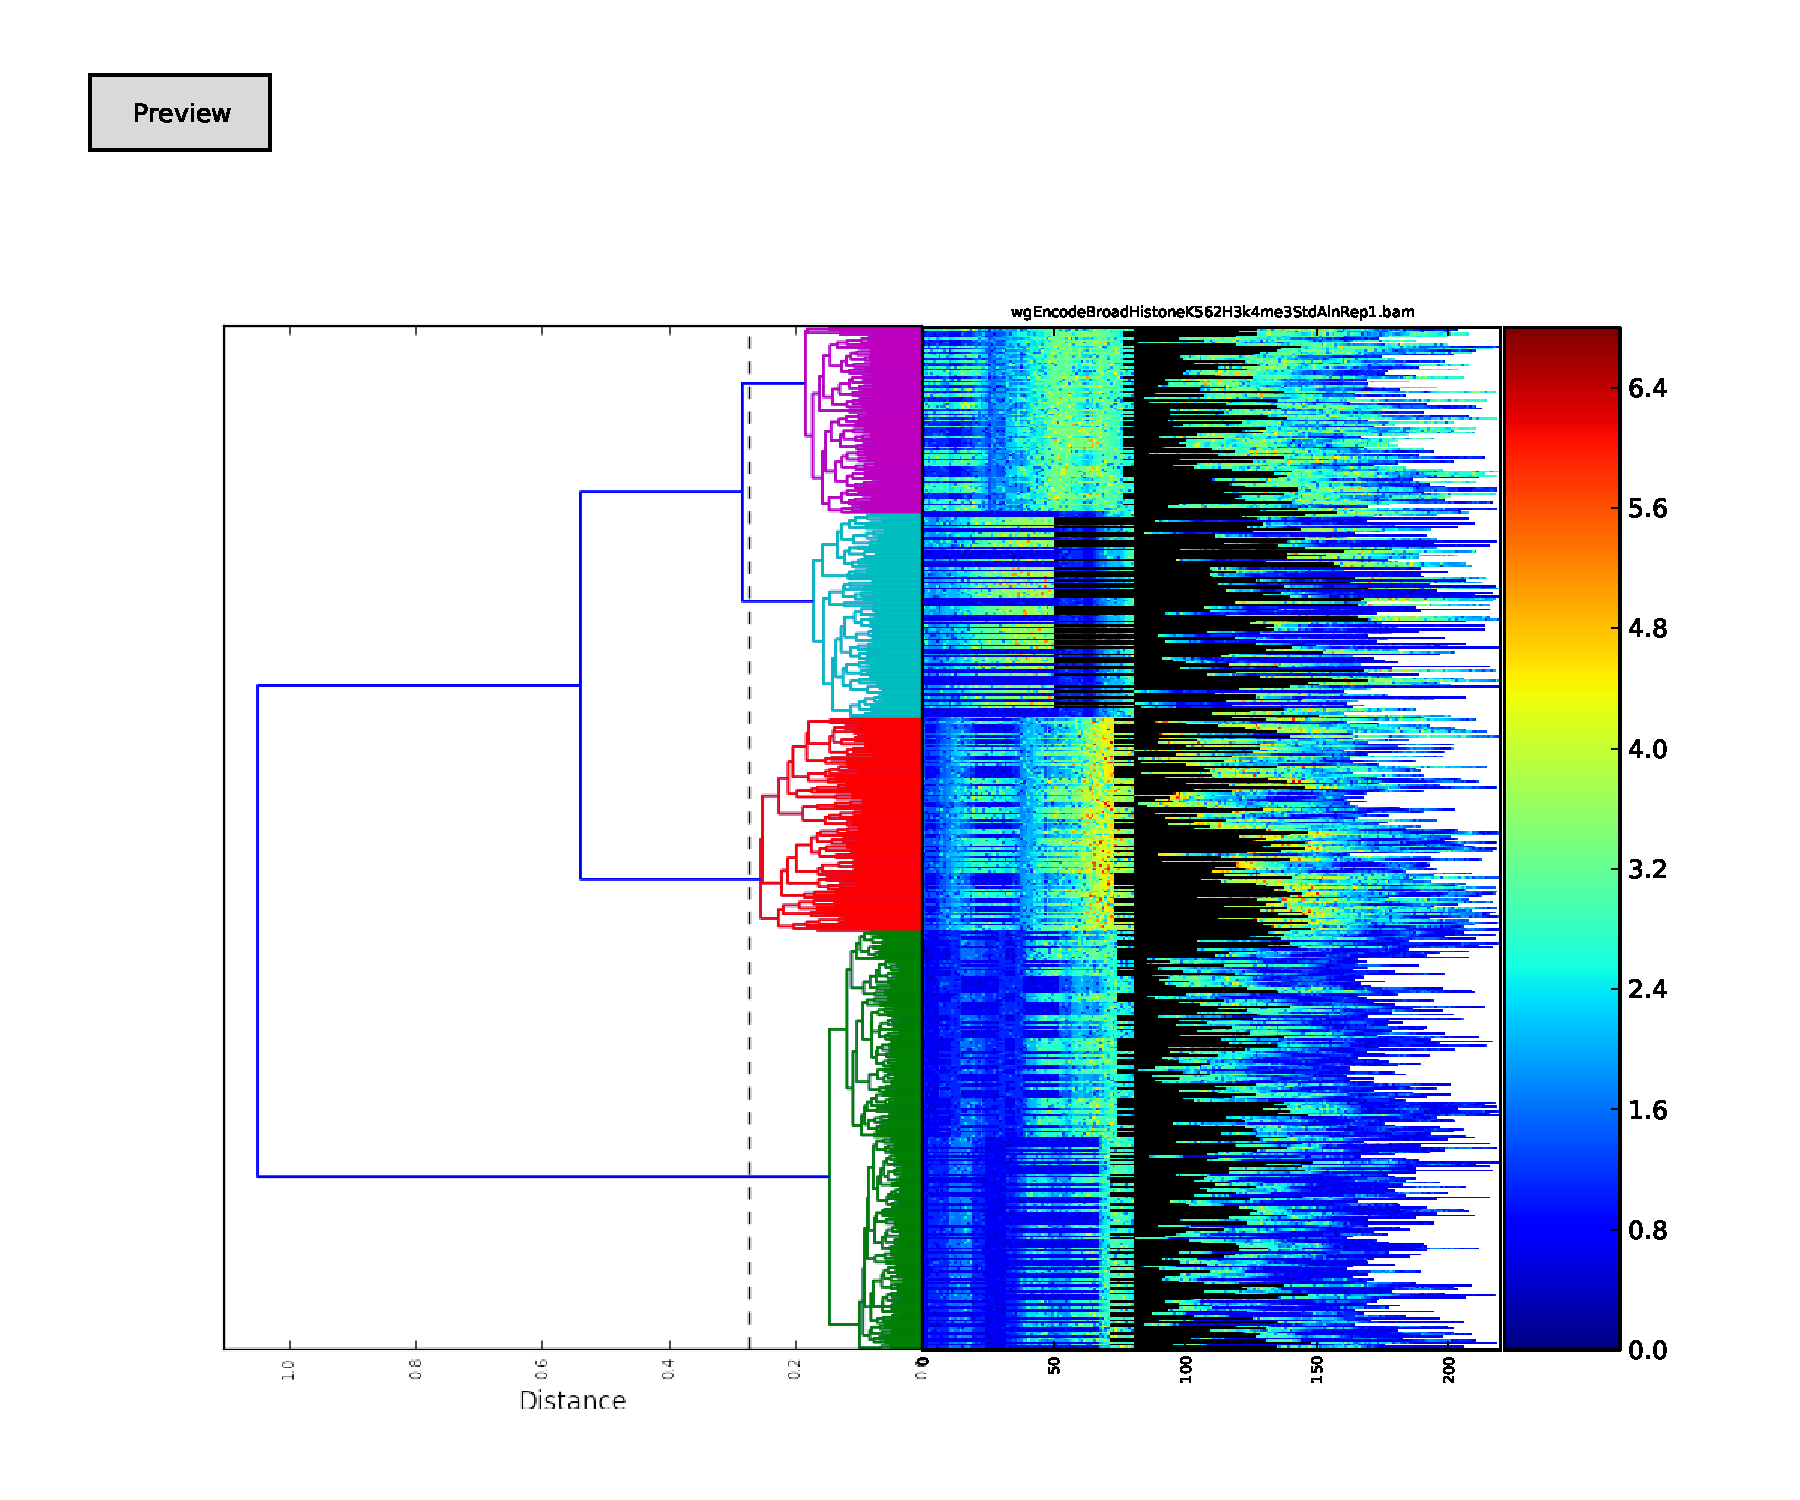
\includegraphics[width=\textwidth]{figures/evaluation/exon_stretching/dgw_cut.pdf}
   \caption{Result of clustering the dataset that was generated by stretching exon regions from the five seed samples in \autoref{fig:evaluation:exon_stretching:seeds}. The extended exons are marked as black points in the heatmap.}
   \label{fig:evaluation:exon_stretching:cut}
\end{figure}

\begin{figure}[t,b]
    \centering
    \begin{subfigure}[b]{0.22\textwidth}
        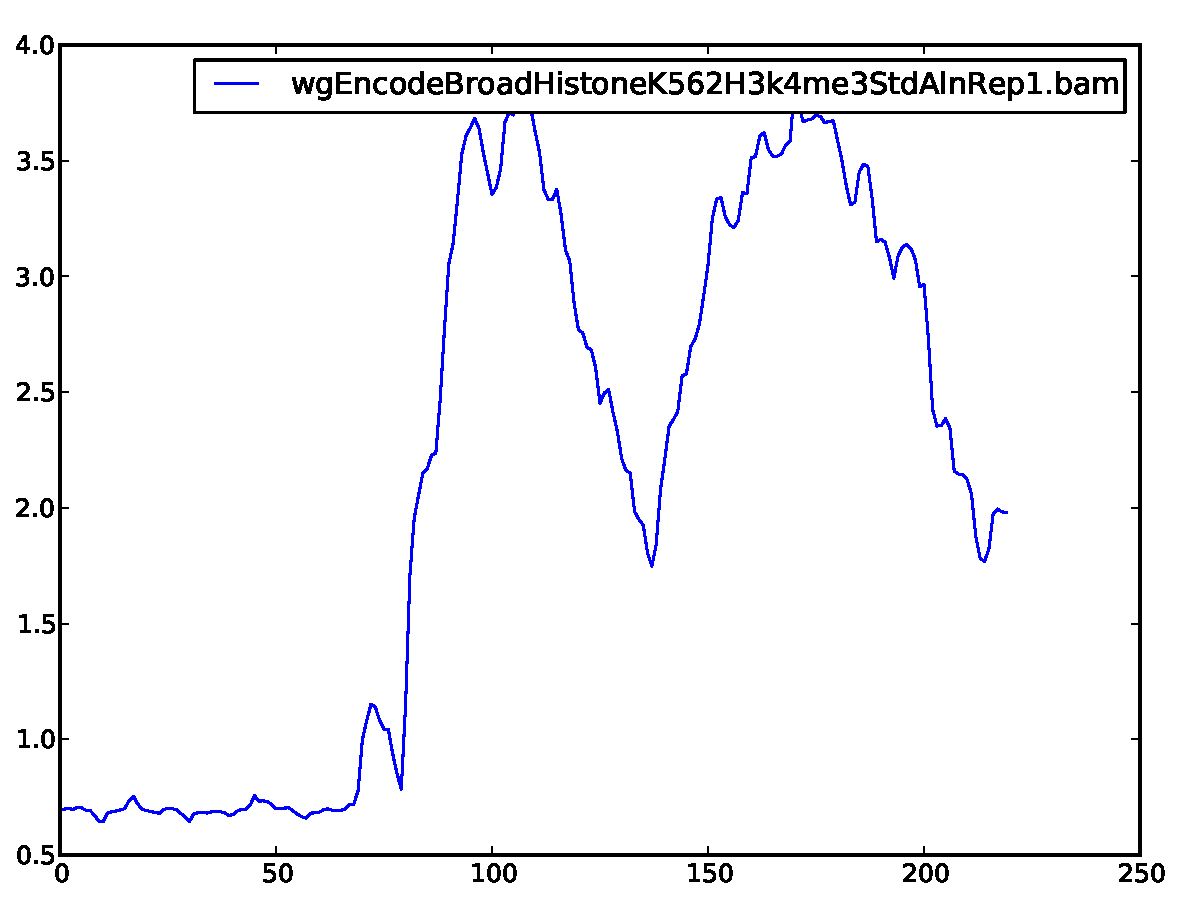
\includegraphics[width=\textwidth]{figures/evaluation/exon_stretching/cluster-1.pdf}
        \caption{Magenta cluster prototype}
        \label{fig:evaluation:exon_stretching:clusters:1:prototype}
    \end{subfigure}
    ~
    \begin{subfigure}[b]{0.22\textwidth}
        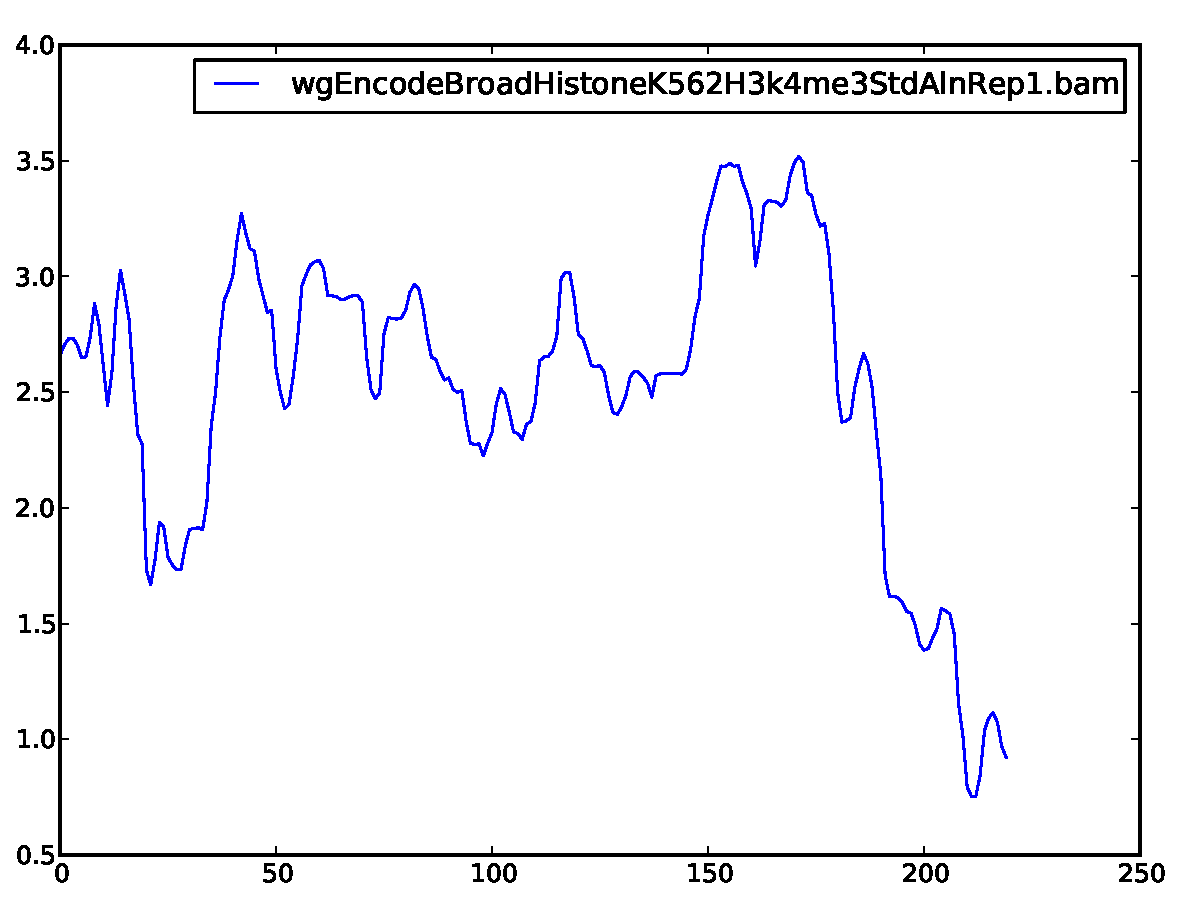
\includegraphics[width=\textwidth]{figures/evaluation/exon_stretching/cluster-2.pdf}
        \caption{Cyan cluster prototype}
        \label{fig:evaluation:exon_stretching:clusters:2:prototype}
    \end{subfigure}
    ~
    \begin{subfigure}[b]{0.22\textwidth}
        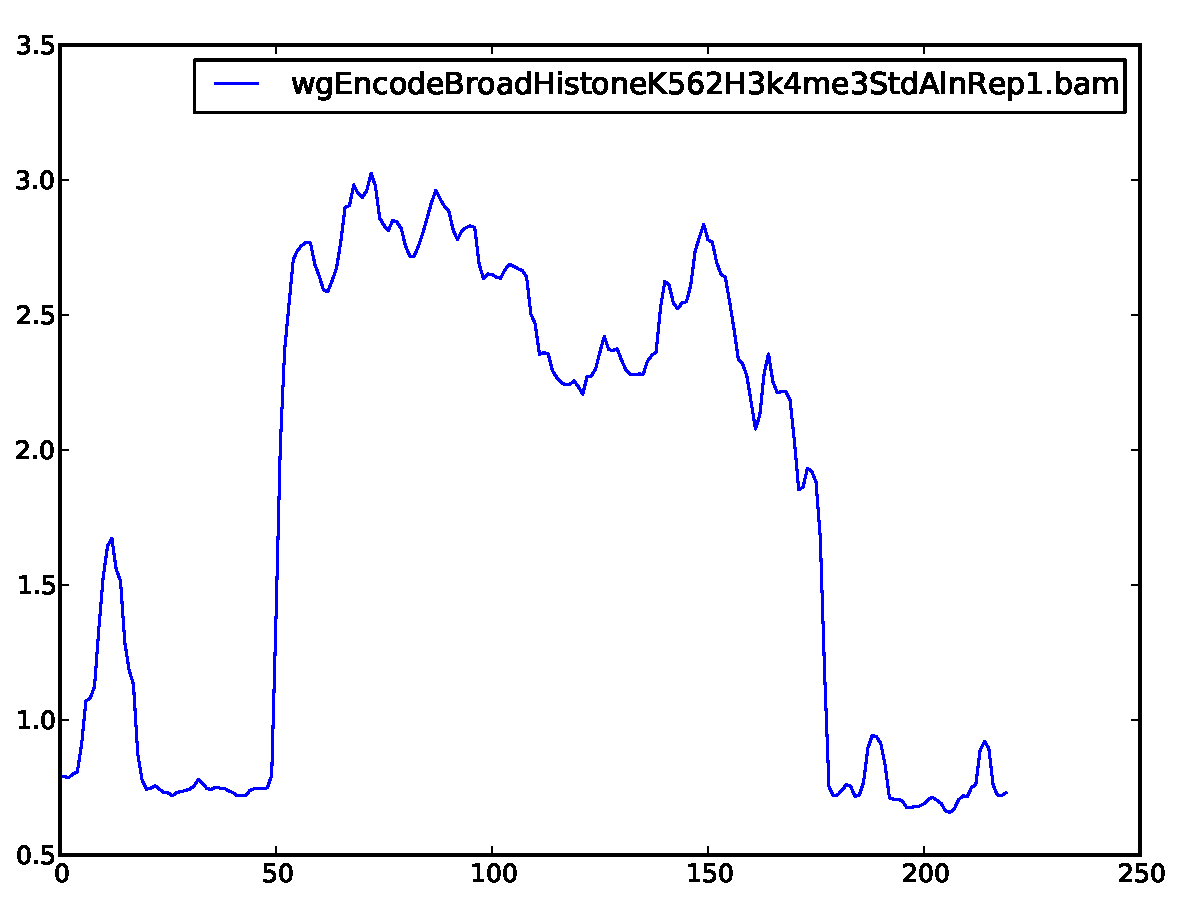
\includegraphics[width=\textwidth]{figures/evaluation/exon_stretching/cluster-3.pdf}
        \caption{Red cluster prototype}
        \label{fig:evaluation:exon_stretching:clusters:3:prototype}
    \end{subfigure}
    ~
    \begin{subfigure}[b]{0.22\textwidth}
        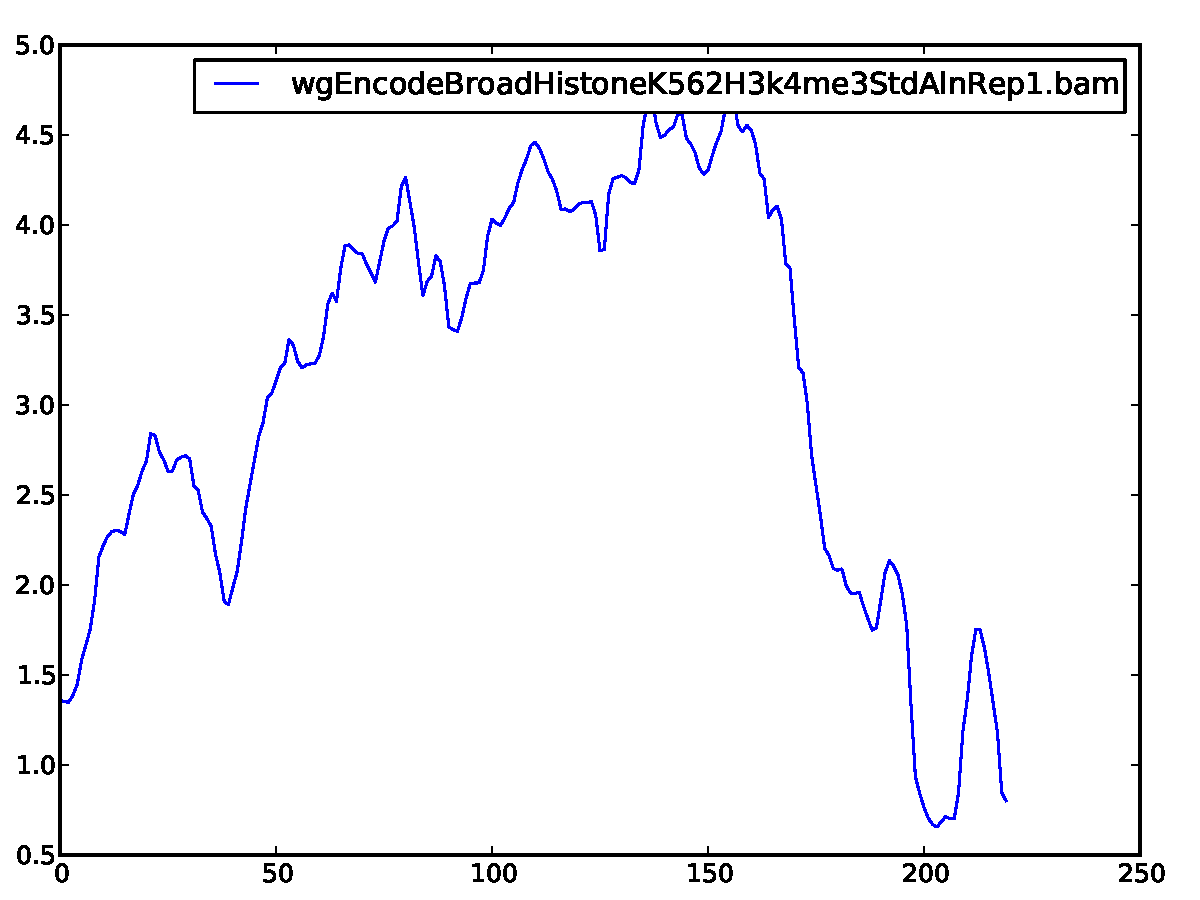
\includegraphics[width=\textwidth]{figures/evaluation/exon_stretching/cluster-4.pdf}
        \caption{Green cluster prototype}
        \label{fig:evaluation:exon_stretching:clusters:4:prototype}
    \end{subfigure}
    \caption{Prototypes of the four clusters resulting from clustering the artificial dataset}
    \label{fig:evaluation:exon_stretching:clusters:prototypes}
\end{figure}


\begin{figure}[t,b]
    \centering
    \begin{subfigure}[b]{0.22\textwidth}
        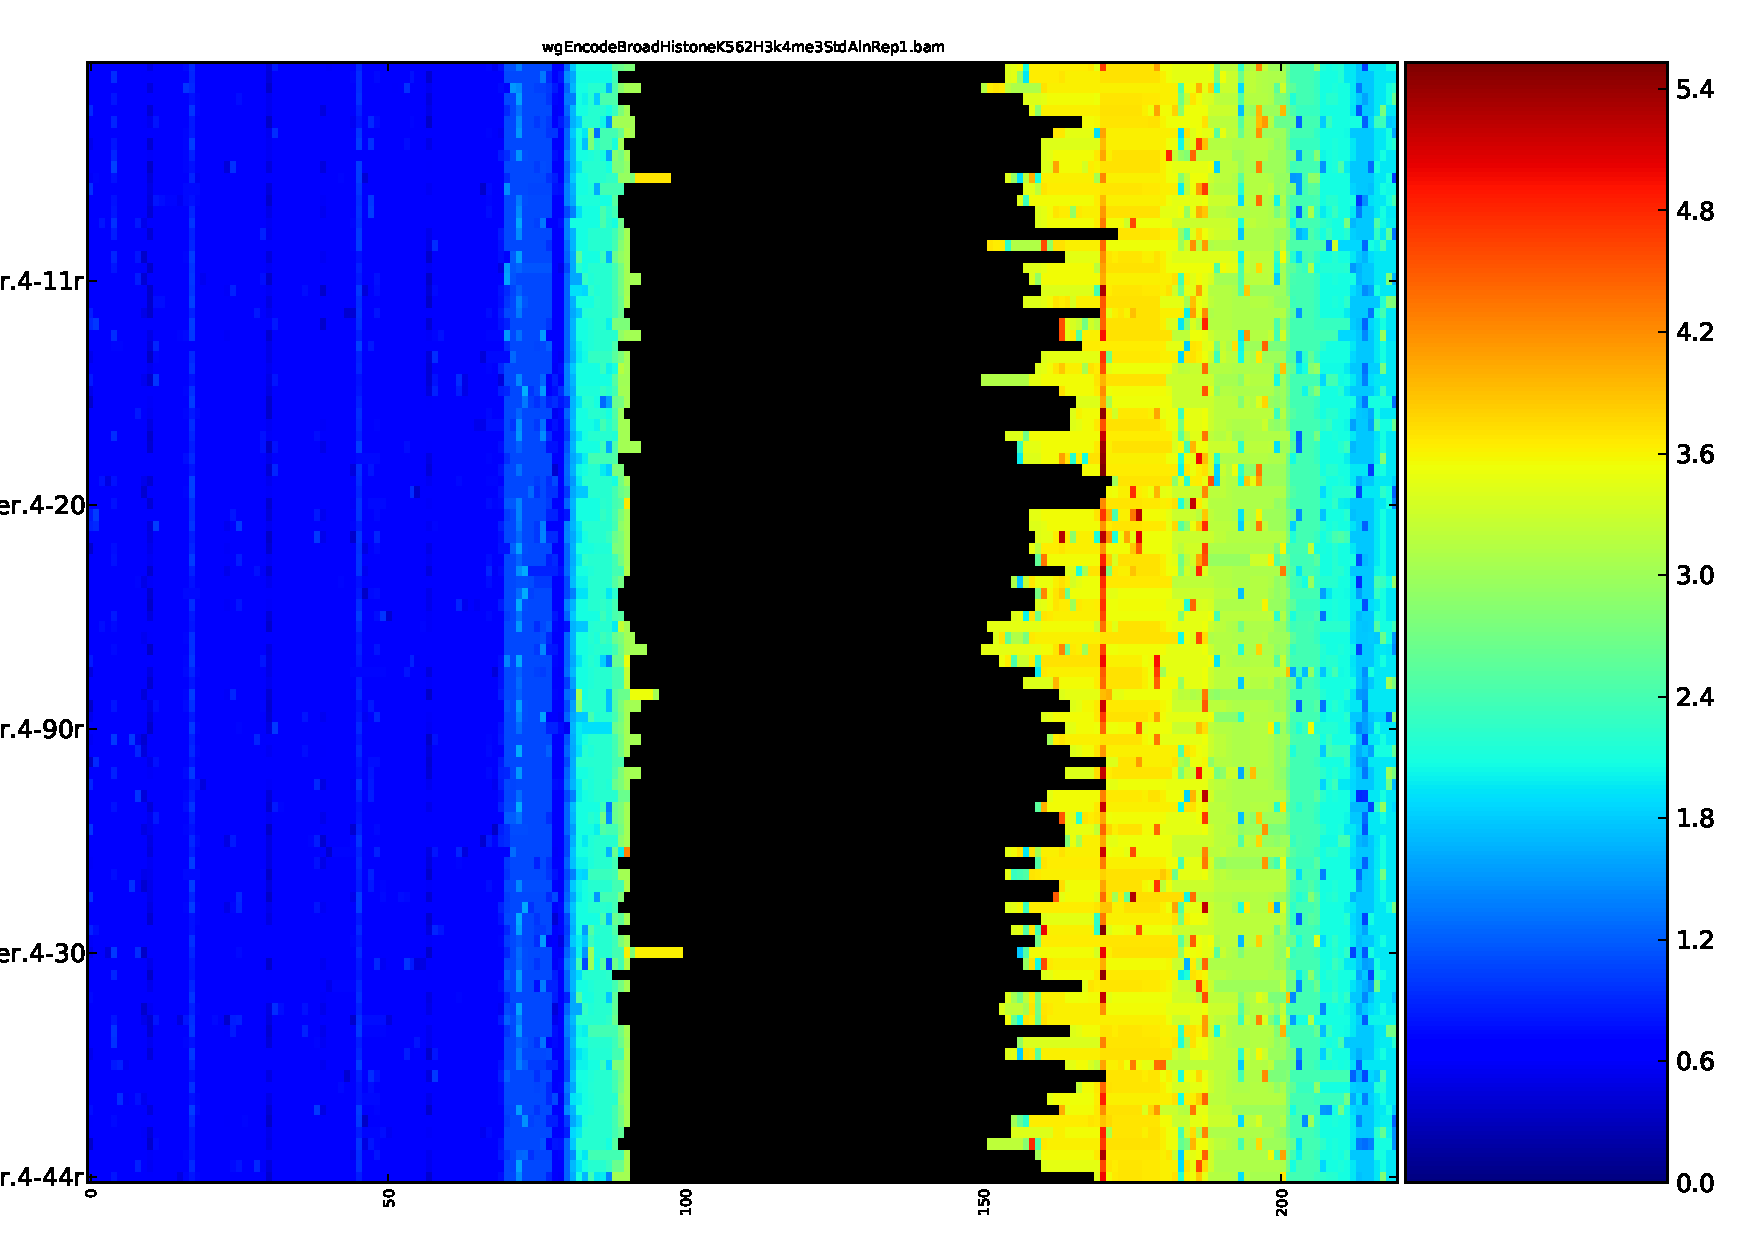
\includegraphics[width=\textwidth]{figures/evaluation/exon_stretching/cluster-warped-1.pdf}
        \caption{Magenta cluster}
        \label{fig:evaluation:exon_stretching:clusters:1:warped}
    \end{subfigure}
    ~
    \begin{subfigure}[b]{0.22\textwidth}
        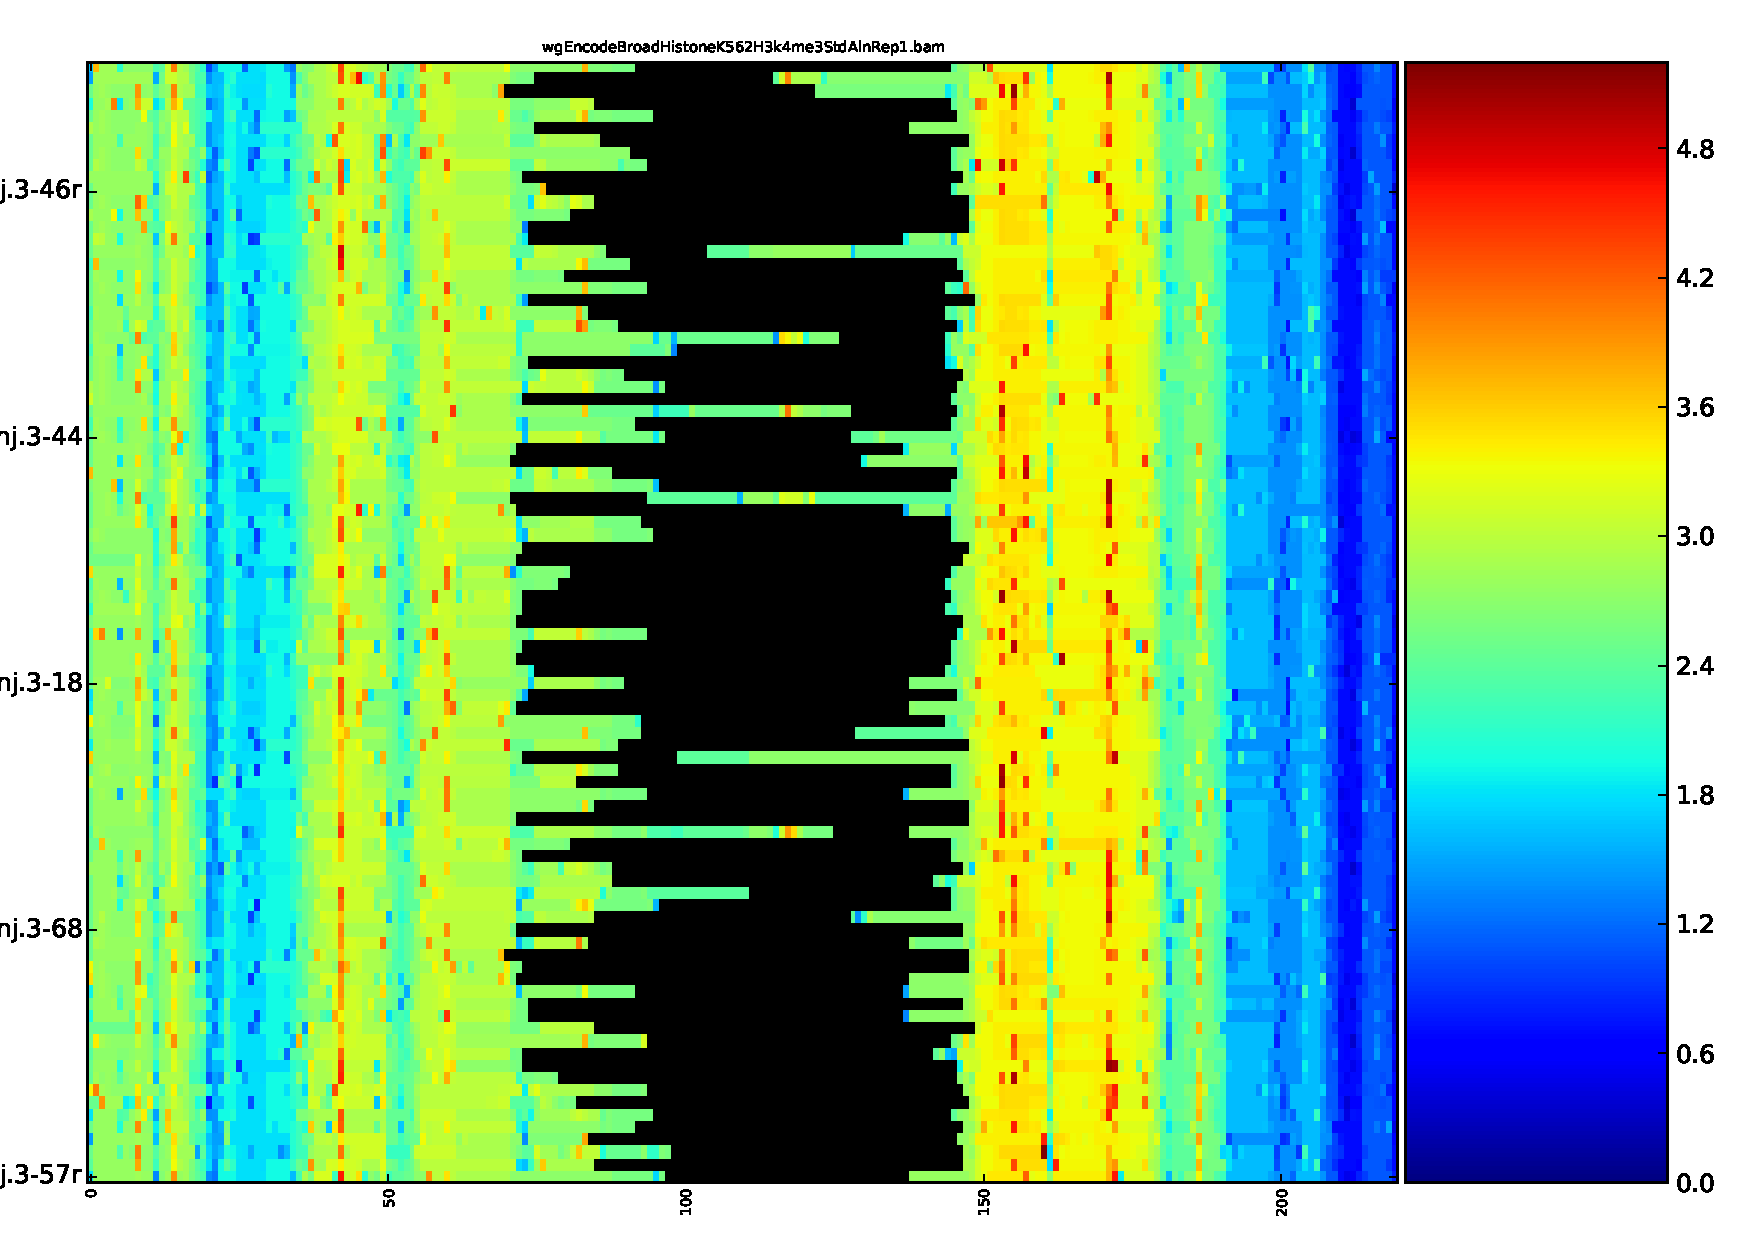
\includegraphics[width=\textwidth]{figures/evaluation/exon_stretching/cluster-warped-2.pdf}
        \caption{Cyan cluster}
        \label{fig:evaluation:exon_stretching:clusters:2:warped}
    \end{subfigure}
    ~
    \begin{subfigure}[b]{0.22\textwidth}
        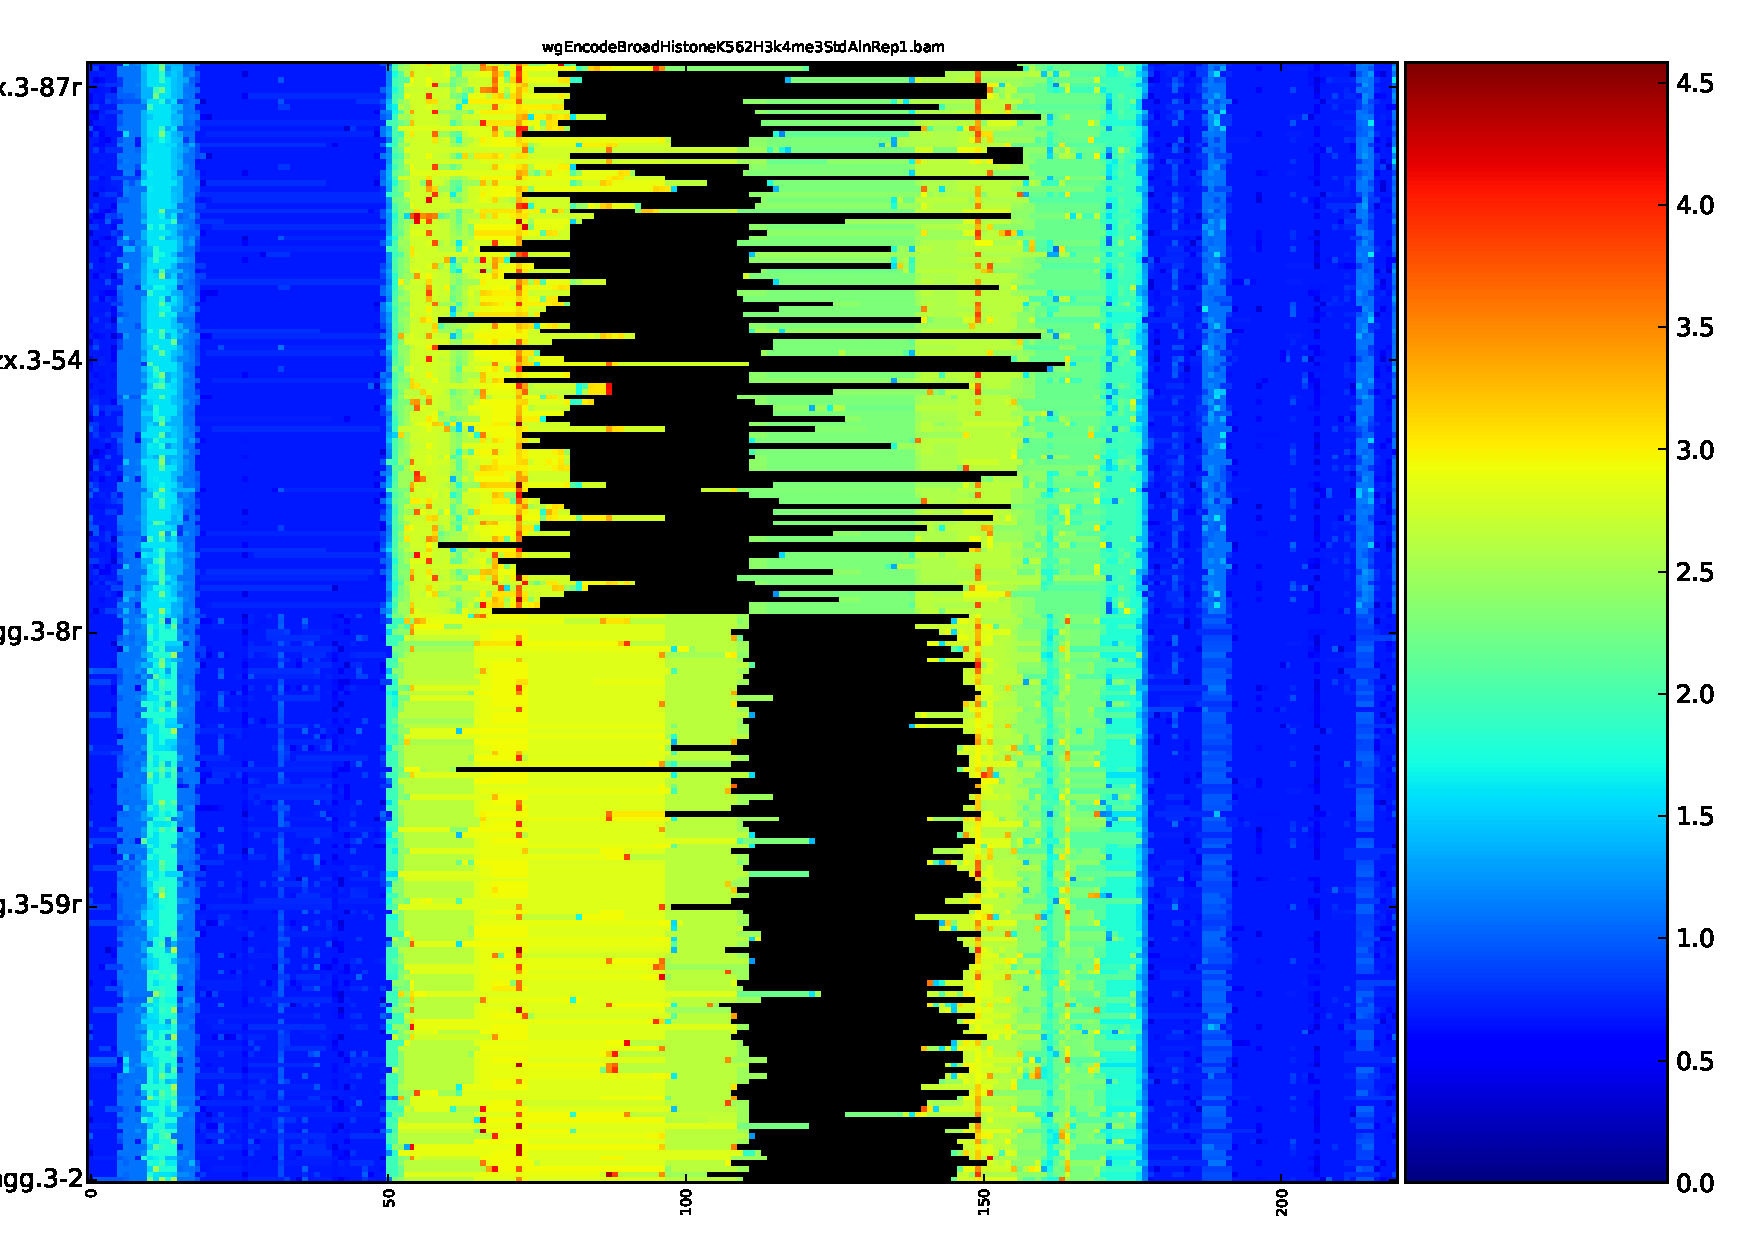
\includegraphics[width=\textwidth]{figures/evaluation/exon_stretching/cluster-warped-3.pdf}
        \caption{Red cluster}
        \label{fig:evaluation:exon_stretching:clusters:3:warped}
    \end{subfigure}
    ~
    \begin{subfigure}[b]{0.22\textwidth}
        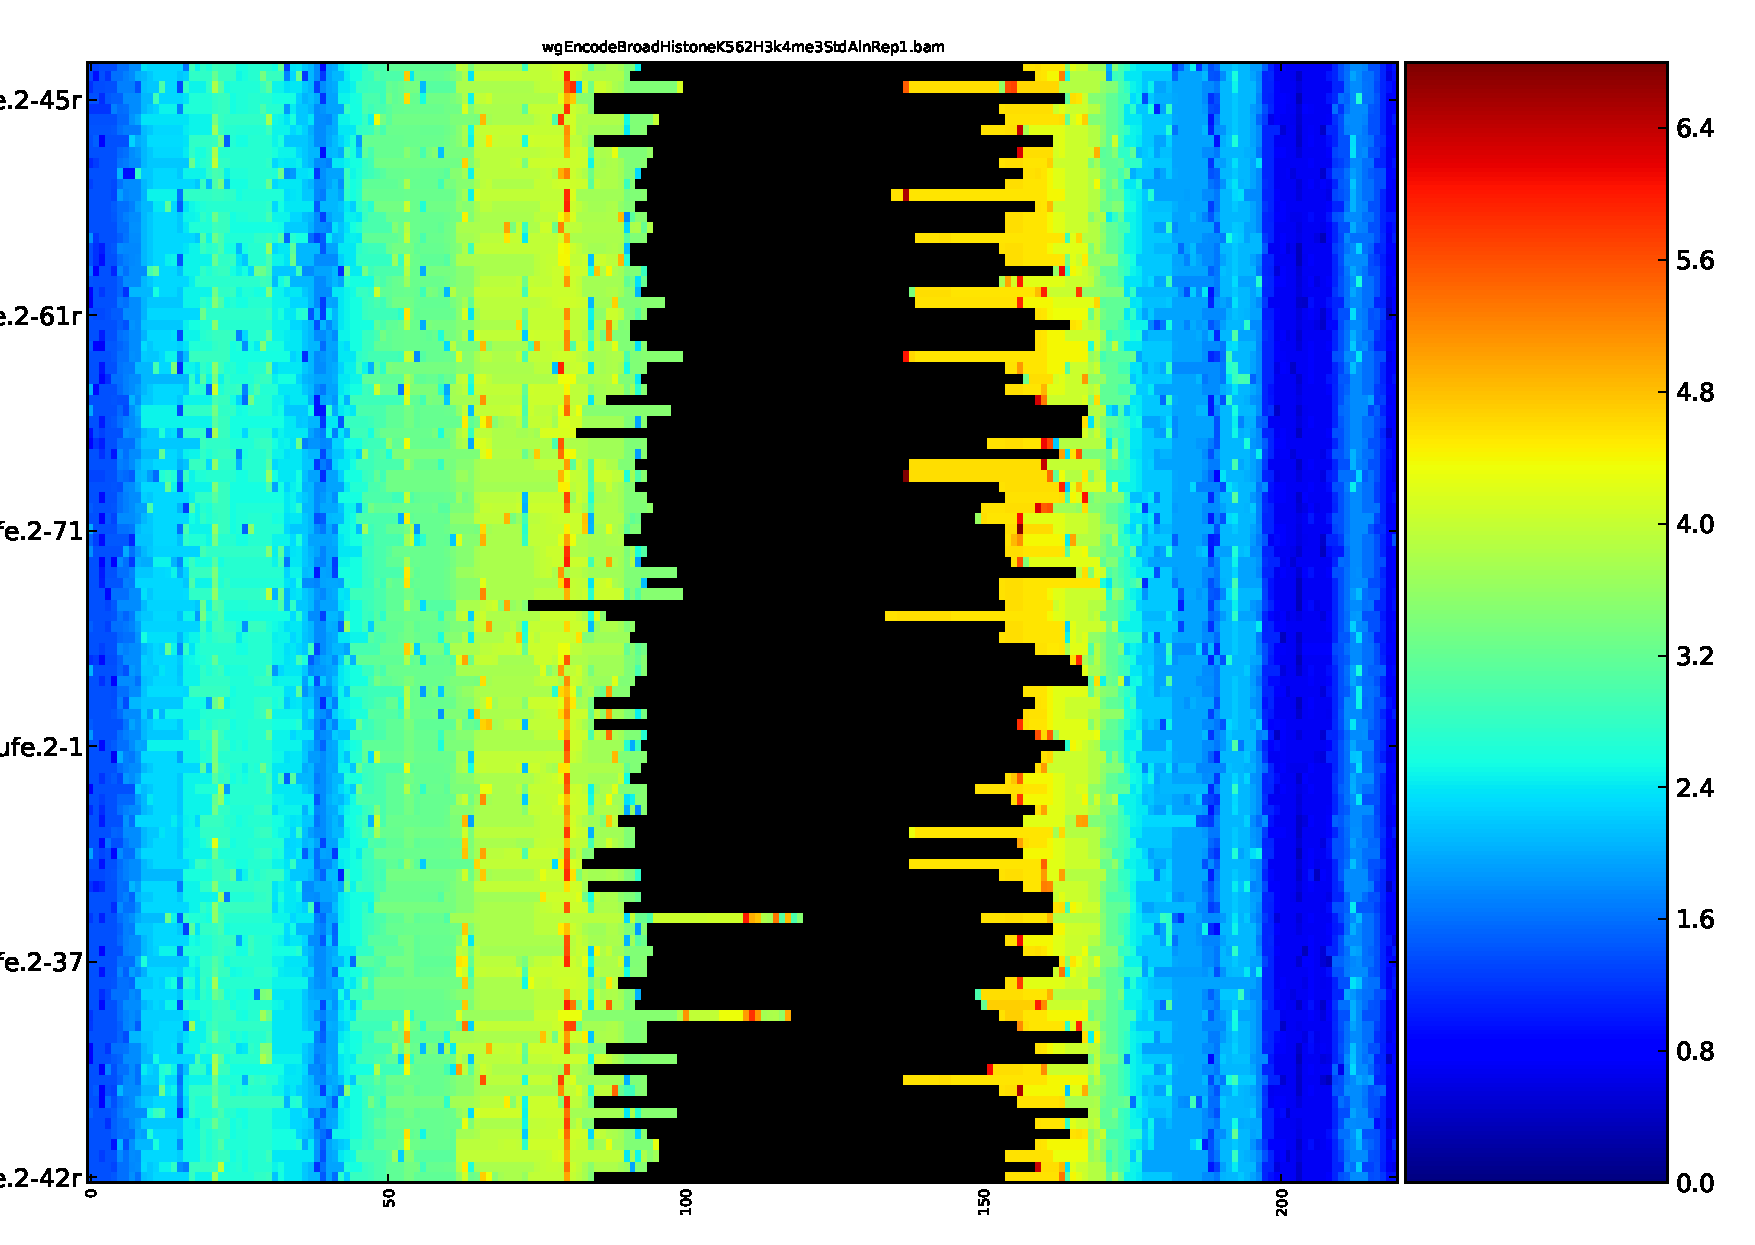
\includegraphics[width=\textwidth]{figures/evaluation/exon_stretching/cluster-warped-4.pdf}
        \caption{Green cluster}
        \label{fig:evaluation:exon_stretching:clusters:4:warped}
    \end{subfigure}
    \caption{Data dynamically warped onto the prototypes.}
    \label{fig:evaluation:exon_stretching:clusters:warped}
\end{figure}

\autoref{fig:evaluation:exon_stretching:cut} shows the resulting hierarchical clustering of these regions. One can see that only four clusters are formed at the cut level chosen by me, not five. 
These clusters are pictured in Figures \ref{fig:evaluation:exon_stretching:clusters:prototypes} and \ref{fig:evaluation:exon_stretching:clusters:warped}. It can be estimated from the prototypes of each of the cluster in \ref{fig:evaluation:exon_stretching:clusters:prototypes} which seed the data was generated from.

The largest, green cluster, was generated from the two similar regions, \gene{uc001nng.3} and \gene{uc001czx.3}. As expected, these two regions were joined early, because of their similarity and the flipping of one of the seed regions can be clearly seen in \autoref{fig:evaluation:exon_stretching:clusters:3:warped}. In fact, from the dendrogram we can see that these two clusters were joined earlier than other clusters were formed. This can be explained remembering that the mutation function used in this experiment is proportional to the value of the actual point, therefore regions having more bins that are relatively unexpressed, such as the ones in figures \ref{fig:evaluation:exon_stretching:seeds:c} and \ref{fig:evaluation:exon_stretching:seeds:d},
will be mutated less, and therefore would be constructed earlier.

\todo{Edit out the preview button maybe from \autoref{fig:evaluation:exon_stretching:cut}?}

\section{Clustering the Results of a Peak Caller}
\label{sec:macs-experiment}
Tests on a artificial benchmark have shown that the DGW algorithm is able to do what it says it does.
However, is the performance of DGW on a real dataset. The DGW was evaluated in the following scenario. MACS peak caller \cite{Zhang:2008wp} was run on the Chip-Seq results for \histonemodification{H3K4Me3} marks in \celltype{K562} cell type. A control sample was used when calling for peaks as to anticipate between significant and insignificant peaks. The remaining parameters of MACS peak caller were left default.

Peaks that are within 50bp of each other, were then merged together using {\\tt BEDTools} package\cite{Quinlan:2010ur}. Then, all transcription start sites and first splicing sites overlapping these regions were found and marked as points of interest. Regions that contain no first splicing sites in them were dropped.

The datasets for \histonemodification{H3K4Me3} and \histonemodification{H3K9Ac} histone modifications for \celltype{K562} were obtained from ENCODE. These modifications were then clustered at the extracted regions of interest using DGW.
The DGW parameters were set to have resolution of 50 base pairs per bin, use squared euclidean distance as a local distance measure, use slanted band constraint of size 12 (see \autoref{sec:slanted-band-constraint} for more information) and normalise the height of read pileups \todo{Need to write about this!}.

The results are visible in \autoref{fig:evaluation:macs-peaks}. \todo{Comment on the results following the paper}.

\begin{figure}
    \centering
    \begin{subfigure}[b]{0.45\textwidth}
         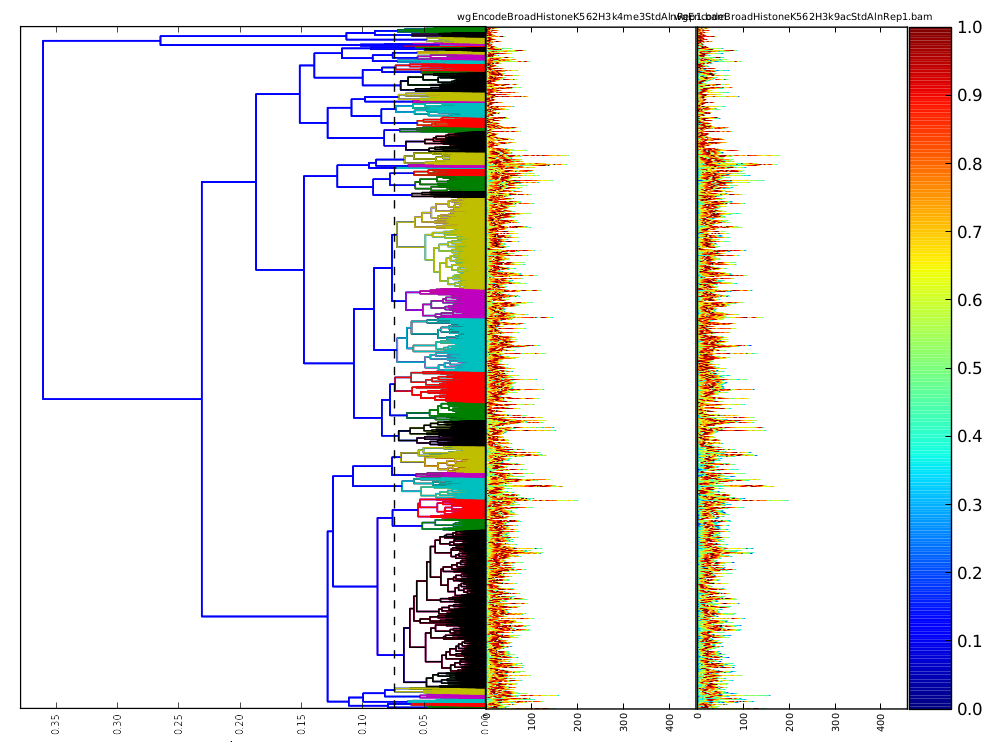
\includegraphics[width=\textwidth]{figures/evaluation/macs-peaks/cut-no-preview-button.png}
         \caption{Resulting Dendrogram}
         \label{fig:evaluation:macs-peaks:cut}
    \end{subfigure}
    ~
    \begin{subfigure}[b]{0.45\textwidth}
        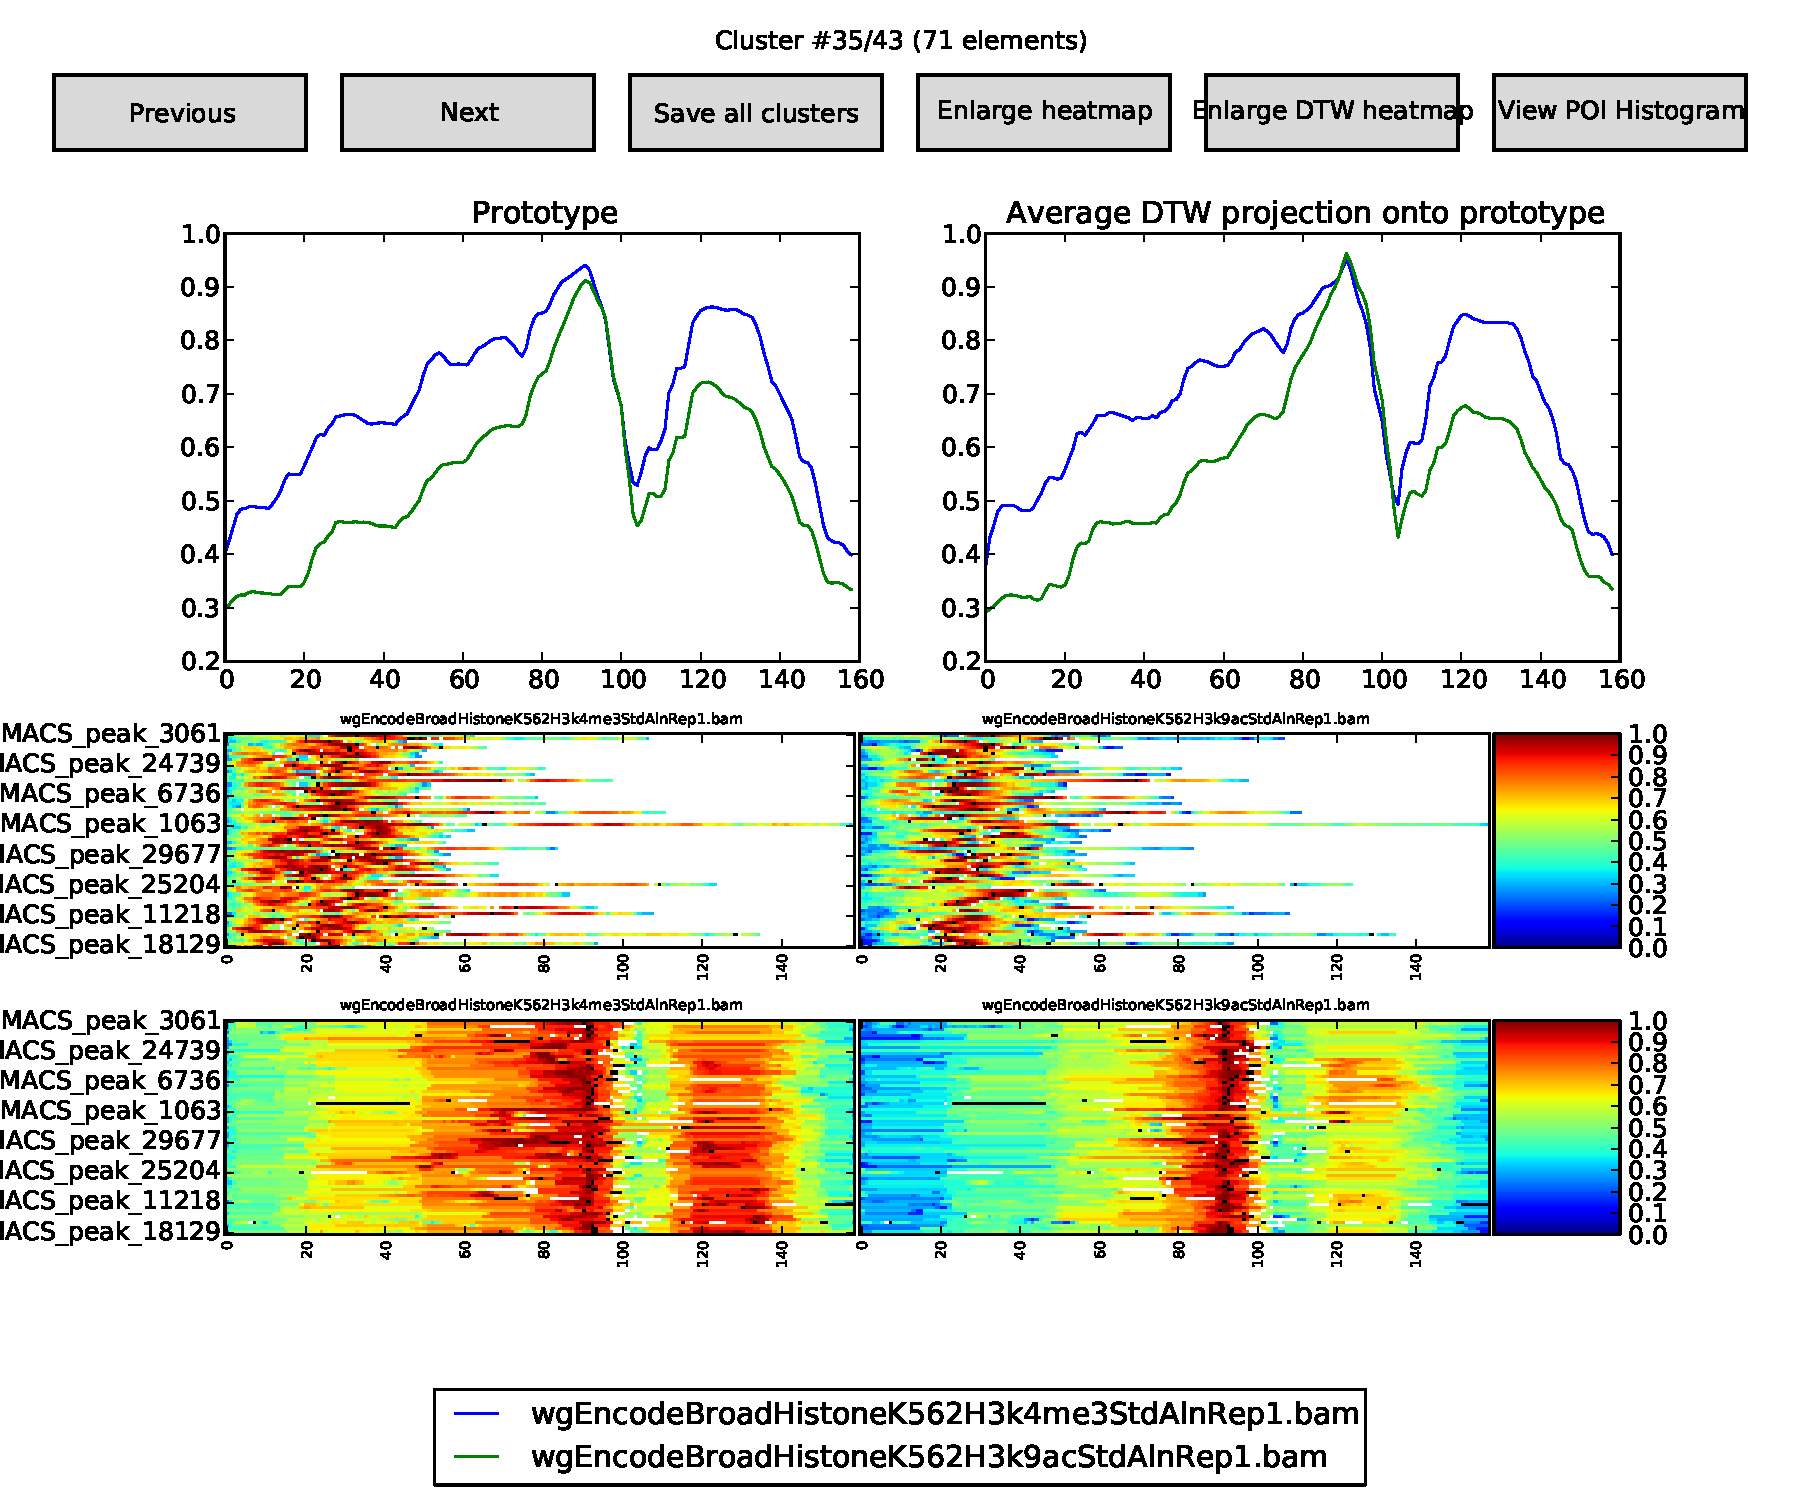
\includegraphics[width=\textwidth]{figures/evaluation/macs-peaks/dgw-explorer-cluster-35.pdf}
        \caption{Explorer window for cluster 35}
        \label{fig:evaluation:macs-peaks:explorer}
    \end{subfigure}
    ~
    \begin{subfigure}[b]{0.45\textwidth}
        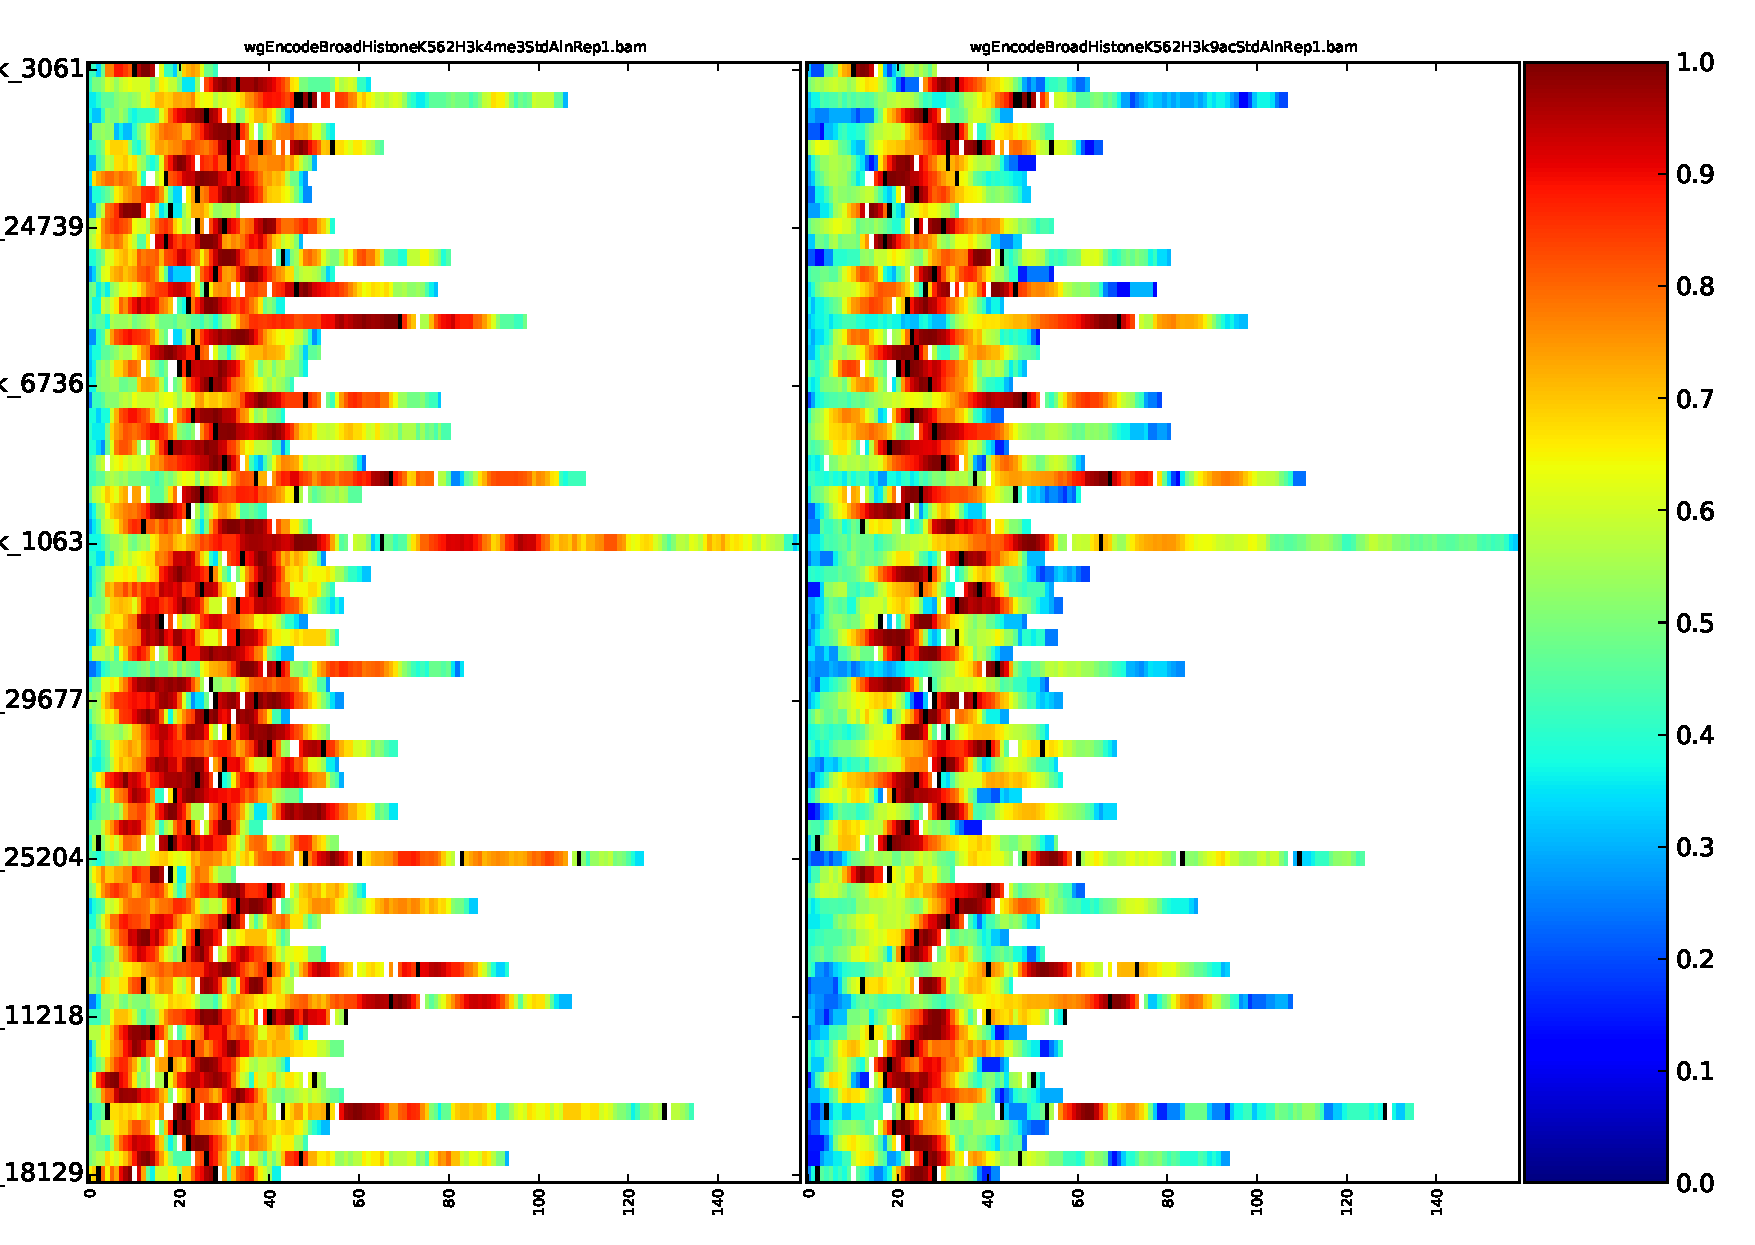
\includegraphics[width=\textwidth]{figures/evaluation/macs-peaks/dgw-cluster-35-original-heatmap.pdf}
        \caption{Heatmap of the original data in the cluster}
        \label{fig:evaluation:macs-peaks:original-heatmap}
    \end{subfigure}
    ~
    \begin{subfigure}[b]{0.45\textwidth}
        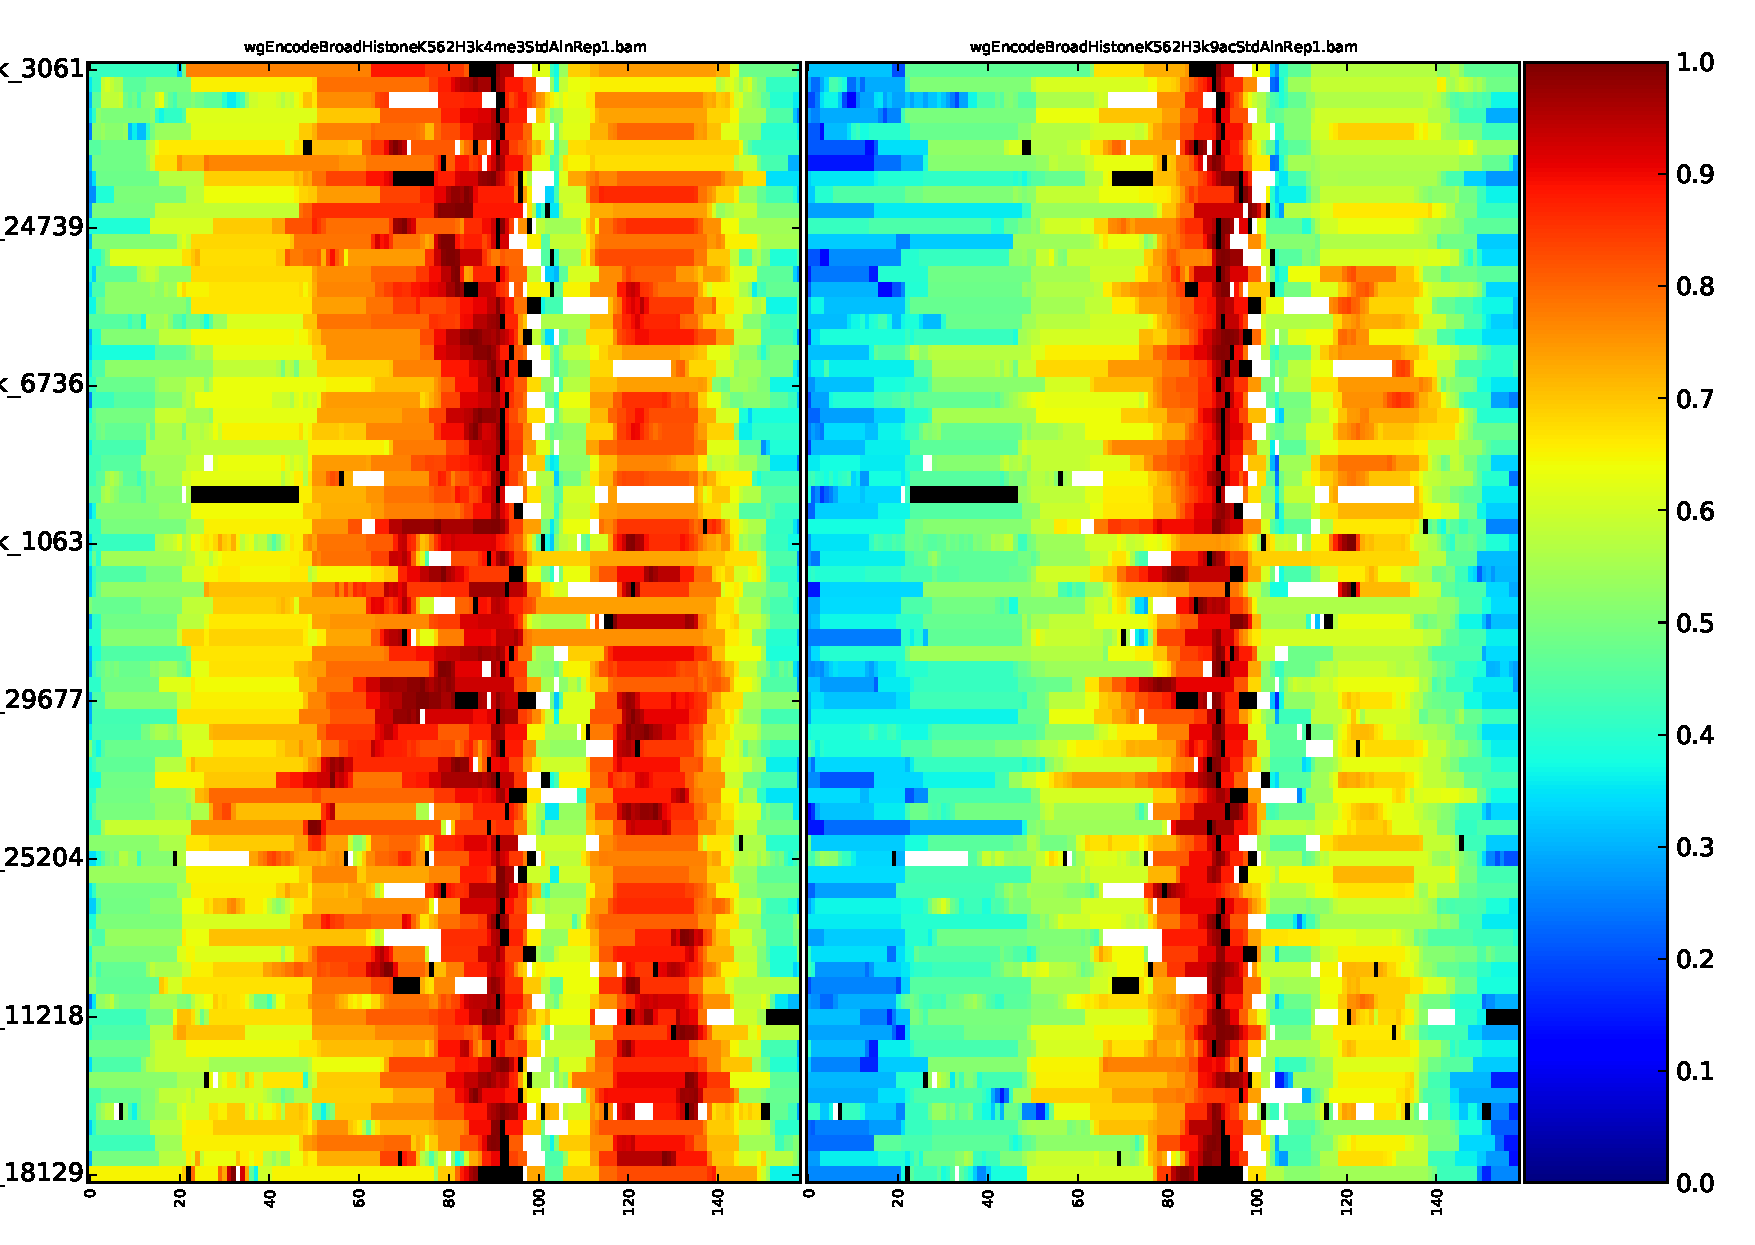
\includegraphics[width=\textwidth]{figures/evaluation/macs-peaks/dgw-cluster-35-warped-heatmap.pdf}
        \caption{Heatmap of the cluster data projected onto the cluster prototype.}
        \label{fig:evaluation:macs-peaks:warped-heatmap}
    \end{subfigure}
    ~
    \begin{subfigure}[b]{0.45\textwidth}
        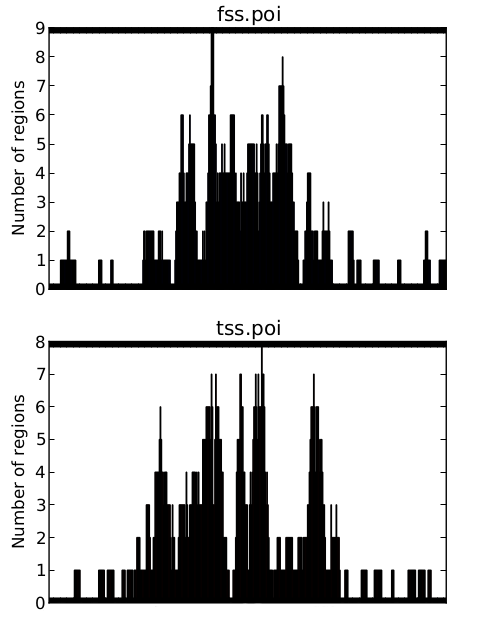
\includegraphics[width=\textwidth]{figures/evaluation/macs-peaks/cluster-35-histogram-clean.png}
        \caption{Distribution of POI per bin before warping.}
        \label{fig:evaluation:macs-peaks:histogram-original}
    \end{subfigure}
    ~
    \begin{subfigure}[b]{0.45\textwidth}
        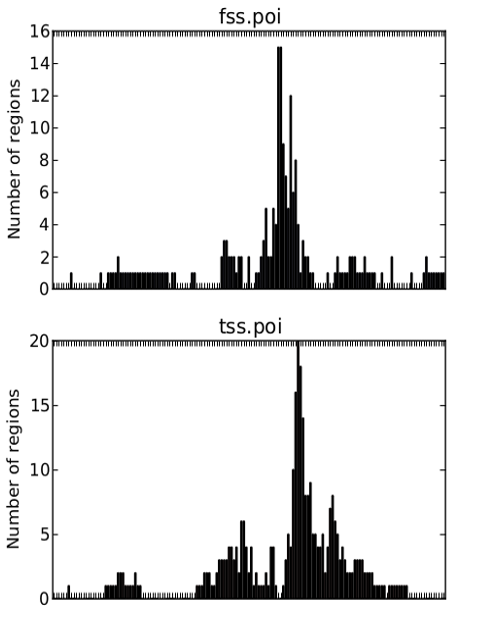
\includegraphics[width=\textwidth]{figures/evaluation/macs-peaks/cluster-35-warped-histogram-clean.png}
        \caption{Distribution of POI per bin after warping.}
        \label{fig:evaluation:macs-peaks:histogram-warped}
    \end{subfigure}
    \caption{Results of clustering the peaks found by MACS peak caller. Transcription start sites are marked in white and the first splicing sites are marked in black in the heatmaps. The two histograms in \ref{fig:evaluation:macs-peaks:histogram-original} and \ref{fig:evaluation:macs-peaks:histogram-warped} show the distribution of the number of regions containing a transcription start site or a first splicing site in each of the bins. For original data, all regions were stretched to be of the same length before calculating the distributions.}
    \label{fig:evaluation:macs-peaks}

    
    
\end{figure}




\todo{Write a list of datasets somewhere in appendix}

\chapter{Conclusions and Contributions}

\bibliographystyle{alpha}
\bibliography{papers2}

\appendix
\todo{Include both papers}

\end{document}
